\documentclass[a4paper,fleqn]{cas-sc}

\usepackage[authoryear,longnamesfirst]{natbib}
\usepackage{booktabs}
\usepackage{graphicx}
\usepackage[protrusion=true,expansion=false]{microtype}
\usepackage[section]{placeins}

\setlength{\textfloatsep}{8pt plus 2pt minus 2pt}
\setlength{\floatsep}{7pt plus 2pt minus 2pt}
\setlength{\intextsep}{7pt plus 2pt minus 2pt}
\setlength{\abovecaptionskip}{4pt}
\setlength{\belowcaptionskip}{2pt}
\setcounter{topnumber}{5}
\setcounter{totalnumber}{8}
\renewcommand{\topfraction}{0.95}
\renewcommand{\textfraction}{0.04}
\renewcommand{\floatpagefraction}{0.80}

\newcommand{\sidetablecaption}[2]{%
  \refstepcounter{table}\label{#1}%
  \begingroup
  \raggedright\footnotesize
  \textbf{Table~\thetable}\par
  #2\par
  \endgroup
  \vspace{3pt}
}
\newcommand{\diagiface}[1]{\emph{#1}\textsuperscript{\dag}}
\RenewDocumentCommand \printorcid { } { }

\begin{document}
\let\WriteBookmarks\relax
\def\floatpagepagefraction{1}
\def\textpagefraction{.001}

\shorttitle{Evidence Interfaces for RAG Readers}
\shortauthors{Anonymous Authors}

\title[mode=title]{Evidence Interfaces Shape How Retrieval-Augmented Readers Learn and Use Context}

\author[1]{Anonymous Author}
\affiliation[1]{organization={Anonymous Institution},
  city={Anonymous City},
  country={Anonymous Country}}

\begin{abstract}
Retrieval-augmented generation systems are usually evaluated by asking whether
the retriever finds relevant evidence. For a reader model, however, evidence
availability is only part of the problem: the same support can be easy or hard
to use depending on how it is ordered, shortened, or represented in the input.
We study this handoff as an \emph{evidence interface}, the reader-facing
representation produced by a retriever, dataset, or selector. Across HotpotQA,
2WikiMultiHopQA, and MuSiQue, we compare raw context, realistic top-$k$
retrieval windows, oracle support, oracle support-first ordering, and
structured evidence under matched reader-adaptation settings. The oracle
support, oracle support-first, and structured variants are diagnostics rather
than deployable retrieval methods; they estimate how much answer quality is
lost when support is present but poorly organized. We find that reorganizing
the evidence changes answer quality, prompt cost, and scaling behavior in
these matched settings. Top-$k$ windows behave like useful compression when
they preserve complete support, but become retrieval-coverage failures when
they drop required evidence. Larger readers and more training data narrow
several diagnostic gaps, but do not remove the ordering and organization
effects in our matched settings. These findings suggest that RAG evaluation
should measure not only retrieval relevance, but also whether the reader-facing
evidence is usable.
\end{abstract}

\begin{highlights}
\item We separate evidence availability from reader-facing evidence usability.
\item We compare realistic retrieval windows with oracle interface diagnostics.
\item Cross-dataset results indicate that evidence organization changes reader performance.
\item Support recall explains when top-$k$ windows are compression or coverage failures.
\end{highlights}

\begin{keywords}
Retrieval-augmented generation \sep question answering \sep evidence representation \sep
multi-hop reasoning \sep parameter-efficient adaptation
\end{keywords}

\maketitle

\section{Introduction}

Retrieval-augmented question answering systems are often built around a simple
pipeline: retrieve relevant documents, place them in the reader input, and
generate an answer. This pipeline makes retrieval quality the natural first
target. If the system does not retrieve the needed evidence, the reader has
little chance of answering correctly. This has motivated a large body of work
on retrieval-augmented generation, dense retrieval, reranking, prompt
compression, and long-context modeling
\citep{lewis2020rag,karpukhin2020dpr,khattab2020colbert,xu2023recomp,jiang2023longllmlingua,liu2023lost}.

Retrieval quality is necessary, but it does not fully determine reader
behavior. A reader can receive a context that contains the right evidence and
still fail to use it. The support may be buried late in a long prompt, split
across distractor documents, surrounded by irrelevant text, or represented in a
form that is hard to learn from under the available adaptation budget. The same
support can become easier to use when it is grouped, moved to a prompt
boundary, shortened, or expressed in a compact structure. The missing question
is therefore not whether evidence exists somewhere in the input, but whether
the reader can use the evidence in the form it is given.

This paper studies that handoff as an \emph{evidence interface}. We define an
evidence interface as the reader-facing representation produced by a retriever,
dataset, or selector: which units are shown, in what order, at what
granularity, and in what format. This separates two failure modes that are
often mixed in RAG evaluations. \emph{Evidence availability} asks whether the
selected context contains the information needed to answer the question.
\emph{Reader usability} asks whether the reader can use that information under
a fixed training and inference procedure. A useful RAG pipeline needs both:
retrieval must preserve support, and the reader-facing interface must make that
support usable.

Figure~\ref{fig:pipeline-overview} summarizes the study design. The same
multi-hop QA example is rendered through several evidence interfaces, adapted
with a matched rank-8 LoRA reader setup, and evaluated with answer metrics and
diagnostic probes that separate evidence access from evidence use.

\begin{figure}[t]
\centering
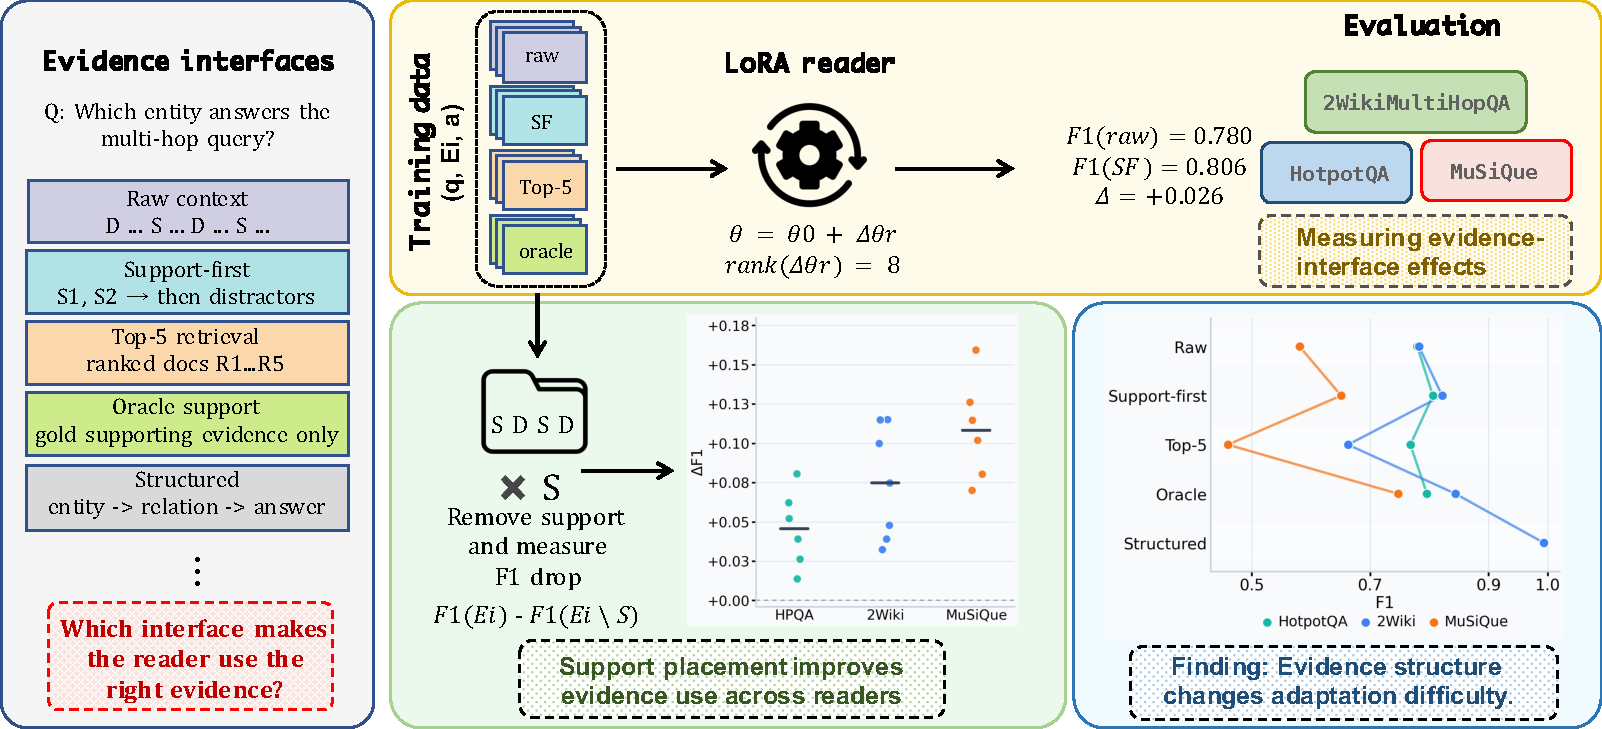
\includegraphics[width=\textwidth]{figs/pipeline.pdf}
\caption{Overview of the evidence-interface study. We render the same QA
examples into multiple reader-facing evidence interfaces, adapt readers with a
matched LoRA setup, and evaluate both answer quality and evidence-use
diagnostics.}
\label{fig:pipeline-overview}
\end{figure}

We evaluate this handoff on three multi-hop QA datasets: HotpotQA,
2WikiMultiHopQA, and MuSiQue
\citep{yang2018hotpotqa,ho2020twowiki,trivedi2022musique}. Multi-hop QA is a
useful testbed because the reader often needs a chain of support units rather
than one isolated passage. For each dataset, we compare raw context,
no-context baselines, realistic retrieval and reranking windows, oracle support
evidence, and oracle support-first diagnostic interfaces. 2WikiMultiHopQA also
provides a structured-evidence diagnostic based on annotated reasoning triples.
These comparisons change the reader input while keeping the question, answer
target, reader family, and adaptation budget matched.

The interfaces have different roles. Raw context is the natural long-input
baseline. Realistic top-$k$ retrieval windows test the tradeoff between prompt
cost and support preservation. Oracle support, oracle support-first ordering,
and structured triples are diagnostics, not deployable retrieval methods. In
particular, oracle support-first uses support annotations to move supporting
units to the front of the context while keeping the raw evidence pool roughly
fixed. Its role is to estimate an interface gap: the answer quality lost when
relevant evidence is present in raw context but poorly organized for the
reader.

Our experiments use parameter-efficient reader adaptation as a measurement
tool. The main setting uses rank-8 LoRA adapters \citep{hu2022lora}, while
training-size sweeps, model-size checks, restricted-adaptation runs, retrieval
support recall, prompt-token cost, answer-likelihood diagnostics,
support-removal tests, and paired error analysis give complementary views of
the same question. LoRA is not the object of study. It gives a controlled
update budget for measuring how hard different evidence interfaces are for the
reader to learn and use.

Across the completed conditions, the oracle diagnostics expose a consistent
interface gap. They score above raw context across datasets and reader
families. The gain is smallest on HotpotQA and larger on 2WikiMultiHopQA and
MuSiQue, where contexts are more diffuse or support coverage is harder. Larger
readers and more training data reduce some gaps, but the matched oracle
contrasts remain positive in the completed settings. Realistic top-5 windows
reduce prompt length substantially. Their interpretation depends on support
recall: the HotpotQA window mostly preserves support and behaves like useful
compression, whereas the 2WikiMultiHopQA and MuSiQue windows often drop
required support and become coverage failures. HotpotQA reliance diagnostics
further indicate that evidence-bearing interfaces help because the reader uses
the supporting documents, not only because the prompt format changes.

These findings suggest a practical design lesson for RAG systems. Retrieval
evaluation should check whether support is available, but system evaluation
should also check whether the reader-facing evidence is usable. Selectors,
rerankers, and compressors should therefore be judged not only by retrieval
score or prompt length, but also by whether they preserve support and arrange it
in a form the reader can exploit.

\paragraph{Contributions.}
This paper makes four contributions:
\begin{itemize}
\item We formulate evidence interfaces as a reader-facing design object and
separate evidence availability from reader usability in RAG question answering.
\item We build a cross-dataset interface comparison spanning raw context,
realistic retrieval windows, oracle support, oracle support-first diagnostics,
and gold structured evidence.
\item We find that evidence organization affects answer quality, prompt cost,
data scaling, and model scaling under matched reader-adaptation settings.
\item We connect retrieval coverage to reader behavior through support recall,
position controls, support-removal diagnostics, and paired error analysis.
\end{itemize}

\section{Related Work}

\subsection{Retrieval-Augmented Question Answering and Evidence Interfaces}

Open-domain and retrieval-augmented QA connects questions with external
evidence before answer generation. Earlier systems combined retrieval with
reading or answer extraction over Wikipedia-scale corpora
\citep{chen2017drqa,ryu2014wikipediaqa,noraset2021wabiqa}. Modern RAG systems
couple generators with retrieved non-parametric evidence \citep{lewis2020rag},
retrieval-augmented pretraining \citep{guu2020realm}, dense retrieval
\citep{karpukhin2020dpr}, and passage-fusion readers \citep{izacard2021fid}.
Other systems integrate retrieval into pretraining, few-shot inference, or
black-box generation \citep{borgeaud2022retro,izacard2023atlas,shi2024replug}.
IPM work also studies retrieval for conversational QA and RAG with historical
dialogue context \citep{li2023gcoqa,mo2026historicalrag}. This literature
establishes the importance of external information. Our question starts at the
handoff point: given an evidence pool or ranked window, what form should the
reader see?

Multi-hop QA makes the interface problem sharper. Datasets such as WikiHop,
HotpotQA, 2WikiMultiHopQA, and MuSiQue require combining information from
multiple units rather than locating one isolated answer sentence
\citep{welbl2018wikihop,yang2018hotpotqa,ho2020twowiki,trivedi2022musique}.
Several methods therefore retrieve reasoning paths, interleave retrieval with
reasoning, or decompose complex questions into smaller steps
\citep{asai2020reasoningpaths,trivedi2023ircot,khot2023decomposed}. These
approaches show that evidence structure matters for multi-hop reasoning. Our
work asks a complementary question: after a dataset, retriever, or oracle
annotation has assembled an evidence pool, what representation should the
reader see?

We use \emph{evidence interface} for that reader-facing representation. The
same support facts can be mixed with distractors, moved to a prompt boundary,
shortened, or represented as structured facts. This framing is close to IPM
work showing that context granularity and input quality affect downstream QA or
generation \citep{cookingcontext2025,song2026ocr}. Our setting is
retrieval-augmented multi-hop QA, where the central issue is not only which
information is retrieved, but how the reader learns and uses the evidence it is
given. This separates retrieval success from the representation that the reader
must actually process.

\subsection{Long-Context Use and Evidence Position}

Long-context language models make it tempting to pass more retrieved text to
the reader and rely on the model to find the useful parts. Prior work shows why
this is not sufficient. Models can be sensitive to where relevant information
appears in a long input, and evidence placed in the middle of a context can be
harder to use than evidence near the beginning or end \citep{liu2023lost}.
Recent long-context RAG studies make the same broad point from a system angle:
larger context windows change the retrieval tradeoff, but they do not remove
the need to reason about retrieval, ordering, and evidence use
\citep{leng2024longcontextrag,lee2024loft}.

Benchmarks and analyses make the same distinction between nominal context
length and usable context. LongBench and RULER evaluate long-context
capabilities \citep{bai2024longbench,hsieh2024ruler}, while other work studies
ordering and recency effects in long inputs
\citep{peysakhovich2023attentionsorting}. These studies warn against treating a
larger context window as a complete solution to evidence use.

Our position controls build on this line of work, but the focus is narrower:
whether the same evidence pool becomes easier or harder for a reader when
support units are buried, grouped, or moved to a stable position. A reader can
fail even when support is present, so support coverage alone does not measure
context usability.

\subsection{Evidence Selection, Reranking, and Compression}

Evidence selection has a long retrieval foundation. Term-based ranking such as
BM25 remains a common baseline \citep{robertson2009bm25}, while dense retrievers
and late-interaction retrievers improve semantic matching
\citep{karpukhin2020dpr,khattab2020colbert}. Cross-encoder rerankers model
query-document interaction more directly and are widely used as a stronger
second-stage ranking signal \citep{nogueira2019bert}. These methods improve
which documents reach the reader, but they do not fully specify how the final
reader input should be organized.

Recent RAG work therefore studies reader-aware selection, compression, and
control. RECOMP and LongLLMLingua compress retrieved evidence
\citep{xu2023recomp,jiang2023longllmlingua}. RankRAG, REPLUG, Self-RAG,
Adaptive-RAG, and corrective RAG connect retrieval choices more directly to
generation behavior \citep{yu2024rankrag,shi2024replug,asai2023selfrag,jeong2024adaptiverag,yan2024crag}.
Related IPM systems explore self-corrective reasoning and adaptive
internal--external knowledge integration \citep{li2026scrag,zhou2026inker}.
In multi-step QA, IRCoT interleaves retrieval with chain-of-thought reasoning
\citep{trivedi2023ircot}.

These methods are complementary to our study. They change retrieval, ranking,
compression, or control policies; we analyze the evidence forms such policies
produce. A window helps only if it preserves support, and a compressed or
structured representation can reduce reader burden while risking information
loss. We therefore report answer quality together with prompt cost and support
recall.

\subsection{Task Formulation and Adaptation Burden}

Our measurement strategy is also related to work showing that the way a task is
formulated can change how difficult it is for a model to learn. A closely
related study analyzes how different reasoning chains affect adaptation
difficulty and intrinsic dimensionality
\citep{prasad2026reasoningchains}. We borrow the controlled-comparison spirit:
hold the model and target task fixed, change the input formulation, and measure
how much adaptation is needed.

Parameter-efficient adaptation provides the experimental tool for this
measurement. Adapter tuning, LoRA, prefix tuning, prompt tuning, and QLoRA show
that large language models can be adapted through small trainable parameter
sets or compact optimization surfaces
\citep{houlsby2019adapters,hu2022lora,li2021prefixtuning,lester2021prompttuning,dettmers2023qlora}.
Related analysis connects fine-tuning success to low-dimensional adaptation
structure \citep{aghajanyan2021intrinsic}. These papers are not about RAG
evidence interfaces, but they motivate using matched adaptation budgets as a
diagnostic for how hard a formulation is to learn.

The present paper uses this idea in a different setting. We do not claim to
estimate a formal intrinsic dimension for each RAG interface. We use LoRA,
training-size sweeps, model-size checks, restricted adaptation runs, and
reliance diagnostics as empirical tools. They tell us whether one evidence
interface is easier for the reader to learn and use than another. This keeps
the contribution at the interface level: evidence organization changes the
reader's usable information, and adaptation behavior is one way to measure that
change.

\section{Methodology}

This section defines the evidence-interface object studied in the paper. The
goal is not to introduce a new RAG architecture. The goal is to make the
retriever--reader handoff explicit enough to evaluate in the same broad
setting as retrieval-augmented readers and passage-fusion QA models
\citep{lewis2020rag,izacard2021fid}. We first formalize the QA setting, then
define the interface design space, the concrete interface families, the reader
adaptation objective, and the diagnostic quantities used in the experiments.

\subsection{Task and Evidence Interface Definition}

Each example is a tuple
\begin{equation}
z_i = (q_i, C_i, S_i, a_i),
\qquad
C_i = (c_{i1}, \ldots, c_{im_i}),
\label{eq:example}
\end{equation}
where $q_i$ is the question, $C_i$ is the candidate evidence pool, $a_i$ is the
reference answer, and $S_i \subseteq C_i$ is the annotated support set when the
dataset provides one. A context unit $c_{ij}$ may be a document, paragraph,
sentence, or dataset-specific structured fact. Some realistic retrieval
interfaces also use a ranking function $R(q_i,C_i)$ over the candidate units;
we write $R_i=R(q_i,C_i)$ when an interface consumes the ranked sequence.

An evidence interface is a reader-facing transformation
\begin{equation}
x_i^{(j)} = I_j(q_i, C_i, S_i, R_i)
          = T(q_i, E_i^{(j)}),
\label{eq:interface-map}
\end{equation}
where $j$ indexes the interface family, $E_i^{(j)}$ is the ordered evidence
sequence selected by the interface, and $T(\cdot)$ is the prompt template that
combines the question with that evidence. The reader then estimates
$p_\theta(a_i \mid x_i^{(j)})$.

This definition separates two properties. \emph{Evidence availability} asks
whether the information needed to answer $q_i$ is present in $E_i^{(j)}$.
\emph{Reader usability} asks whether the trained reader can use the presented
sequence. Two interfaces may contain the same support set while differing in
where support appears, how much distractor text remains, and whether evidence
is expressed as raw text or as a compact structure. Our controlled comparisons
hold $q_i$, $a_i$, the reader family, and the adaptation budget fixed while
changing $I_j$.

\subsection{Methodological Workflow}

The study follows one workflow for every dataset and model. We normalize each
dataset into evidence units and construct one prompt set per interface. We then
adapt a reader separately for each interface, evaluate on the same held-out
questions, and compute matched contrasts. These contrasts are designed to
distinguish missing evidence, poor organization, prompt length, and adaptation
burden. The workflow is intentionally conservative: answer targets, validation
questions, reader family, and adaptation budget are fixed while the
reader-facing interface changes. The main comparisons are therefore controlled
measurements rather than a RAG leaderboard.

\subsection{Evidence Interface Design Space}

We describe an interface through four design axes.

\paragraph{Selection.}
The interface decides which units from $C_i$ are shown. Raw context keeps the
available pool, oracle support keeps only $S_i$, and top-$k$ retrieval windows
keep the highest-ranked units under $R$.

\paragraph{Ordering.}
The interface decides the order of selected units. Raw context uses the dataset
or retriever order. Oracle support-first keeps the raw pool but moves annotated support
to the front of the context. Position controls move the same support block to the
front, middle, or end. These controls are motivated by evidence-position
effects observed in long-context models \citep{liu2023lost}.

\paragraph{Granularity.}
The unit shown to the reader may be a document, paragraph, sentence, or
structured fact. Granularity changes both prompt length and the amount of
irrelevant text surrounding a support fact.

\paragraph{Representation.}
The evidence can remain natural text, be shortened to oracle support text, or be
converted into a structured form when annotations allow it. We treat structured
evidence as a diagnostic upper bound unless such structure is available in the
deployment setting. The shortened-evidence variants are related to retrieval
compression work, but here they are used as controlled diagnostics rather than
as learned compressors \citep{xu2023recomp,jiang2023longllmlingua}.

\subsection{Interface Construction}

Table~\ref{tab:interface-families} summarizes the interface families. In the
table, $\Vert$ denotes sequence concatenation, and $C_i \setminus S_i$ denotes
the raw candidate sequence with support units removed.
$\operatorname{Top}_k(R(q_i,C_i))$ denotes the top-$k$ units returned by a
ranker. $G_i$ denotes a dataset-specific structured evidence object such as the
2WikiMultiHopQA reasoning triples.

\begin{table}[!htbp]
\centering
\caption{Evidence interface families used in the study. Dagger-marked families
use gold support annotations or gold structure and are diagnostic rather than
deployable retrieval interfaces.}
\label{tab:interface-families}
\small
\setlength{\tabcolsep}{3.2pt}
\begin{tabular}{>{\raggedright\arraybackslash}p{0.17\textwidth}
                >{\raggedright\arraybackslash}p{0.28\textwidth}
                >{\raggedright\arraybackslash}p{0.16\textwidth}
                >{\raggedright\arraybackslash}p{0.31\textwidth}}
\toprule
Family & Construction & Status & Role in the study \\
\midrule
No context & $E_i=\varnothing$; question only &
Non-oracle baseline &
Lower-bound baseline for question priors and parametric knowledge. \\
Raw context & $E_i=C_i$ in the dataset or retriever order &
Non-oracle interface &
Main long-context baseline. \\
\diagiface{Support-first} & $E_i=S_i \Vert (C_i \setminus S_i)$ &
Oracle diagnostic &
Oracle diagnostic for the interface gap at roughly fixed length. \\
\diagiface{Oracle support} & $E_i=S_i$ &
Oracle diagnostic &
Clean-evidence upper bound. \\
Retrieval windows & $E_i=\operatorname{Top}_k(R(q_i,C_i))$ &
Non-oracle retrieval window &
Realistic prompt-budget baseline. \\
\diagiface{Structured evidence} & $E_i=G_i$, such as 2Wiki reasoning triples &
Oracle diagnostic &
Diagnostic test of compact evidence structure. \\
\diagiface{Position and distractor controls} & Same support, moved or mixed with distractors &
Oracle diagnostic &
Mechanism checks for position and noise. \\
\bottomrule
\end{tabular}
\end{table}

The oracle diagnostics and deployable-style interfaces answer different
questions. Oracle support-first, oracle support, and structured triples require
support annotations or gold structures; they estimate how much answer quality
is lost when relevant evidence is present but poorly organized. Retrieval
windows instead estimate what realistic ranking and truncation can achieve
under a prompt budget. The paper's central claims come from these contrasts,
not from treating any single interface as the proposed system. Accordingly, the
main tables should be read by interface status first: non-oracle rows describe
deployable-style inputs, while dagger-marked rows describe diagnostic
counterfactuals built from gold labels or gold structure.

\subsection{Reader Adaptation Objective}

For each interface family $j$, we train a reader on prompts
$x_i^{(j)}$ and answer targets $a_i$. The supervised objective is
\begin{equation}
\mathcal{L}_j(\Delta\theta)
= -\frac{1}{N}\sum_{i=1}^{N}
\log p_{\theta_0+\Delta\theta}(a_i \mid x_i^{(j)}),
\label{eq:reader-loss}
\end{equation}
where $\theta_0$ is the frozen base reader and $\Delta\theta$ is the trainable
adapter update for the interface being evaluated.

The main experiments use LoRA as the controlled update budget
\citep{hu2022lora}. For a base weight matrix $W$, the adapted weight is
$W'=W+\Delta W$ with
$\Delta W=(\alpha/r)BA$, where $A$ and $B$ are rank-$r$ trainable matrices.
Unless stated otherwise, $r=8$. LoRA is not the object of study; it fixes the
adaptation budget so that differences across interfaces reflect the difficulty
of learning and using the presented evidence under comparable training
conditions. Rank sweeps and restricted-adaptation runs are used only as
diagnostics for adaptation burden, following the broader idea that controlled
adaptation budgets can expose formulation difficulty
\citep{prasad2026reasoningchains,aghajanyan2021intrinsic}.

Each interface has its own training set because the reader input distribution
changes with $I_j$. A raw-context reader must learn to find support inside a
noisy sequence, while an oracle-support reader mostly maps concise evidence to
the answer. Training separate adapters makes this difference visible and lets
us interpret low-rank adaptation as a measurement of interface cost rather than
as a claim that LoRA is the best adaptation method for RAG. The measured effect
therefore combines two factors: how easily a reader can learn an interface, and
how well it can use that interface at inference time. It should not be read as
a pure format-only comparison under one fixed adapter.

\subsection{Diagnostic Quantities}

We evaluate answer quality with exact match and token-level F1. The methodology
also uses four interface-specific diagnostics. These diagnostics are read
together: paired contrasts isolate question-level changes, support recall checks
whether evidence survives selection, prompt cost records the budget, and
reliance tests whether evidence-bearing gains depend on annotated support.

\paragraph{Matched interface contrasts.}
For any metric $M$ and two interfaces $j$ and $\ell$, we compute matched
question-level differences by averaging
$M(y_i^{(j)},a_i)-M(y_i^{(\ell)},a_i)$ over the same validation questions,
where $y_i^{(j)}$ is the answer generated by the reader trained and evaluated
under interface $j$. The paired bootstrap intervals in the results are based
on these matched differences. This matters because many questions are easy or
hard regardless of interface; paired comparisons focus on whether the same
question changes when evidence is reorganized.

\paragraph{Interface gap.}
The oracle support-first gap measures the gain from reorganizing the same raw
evidence pool with oracle support placement,
$\Delta_{\mathrm{sf-raw}}=\mathrm{F1}(I_{\mathrm{sf}})-\mathrm{F1}(I_{\mathrm{raw}})$.
Because oracle support-first keeps the raw pool roughly fixed, this gap
estimates reader-usability loss rather than a retrieval miss.

\paragraph{Complete-support recall.}
For a top-$k$ retrieval window, we measure whether all annotated support units
survive truncation:
\begin{equation}
\mathrm{Recall@}k
= \frac{1}{N}\sum_{i=1}^{N}
\mathbf{1}\!\left[S_i \subseteq E_i^{\mathrm{top}k}\right].
\label{eq:support-recall}
\end{equation}
This separates retrieval coverage from reader usability. A low-F1 top-$k$
window with low complete-support recall is a retrieval-coverage failure before
it is a reader-interface failure. The support unit follows each dataset's
annotation granularity, so recall values are coverage diagnostics within a
dataset rather than directly comparable measures of identical unit difficulty
across datasets.

\paragraph{Prompt cost.}
We report the average token length of reader inputs,
$\mathrm{Cost}(I_j)=N^{-1}\sum_i |x_i^{(j)}|_{\mathrm{tok}}$. Cost is
interpreted jointly with answer quality and support recall. A short interface
is useful only if it preserves the evidence needed for the answer.

\paragraph{Adaptation scaling.}
To separate interface quality from training-data scarcity, we repeat selected
conditions across training sizes. For training size $n$, we inspect
$G_n(j,\ell)=\mathrm{F1}_n(I_j)-\mathrm{F1}_n(I_\ell)$, especially for raw
context versus oracle support-first or oracle support. If raw context mainly
lacked data, $G_n$ should shrink as $n$ grows. If the gap persists, the
interface itself remains harder for the reader to use.

\paragraph{Evidence reliance.}
For HotpotQA, we also remove annotated support from an evidence-bearing
interface and re-evaluate the trained reader. Let $\bar{S}_i$ denote the
evidence units removed by this ablation; when annotations are finer than the
current context unit, we remove the containing unit so that annotated support is
not left in the prompt:
\begin{equation}
x_{i,-S}^{(j)} = I_j(q_i, C_i \setminus \bar{S}_i, \varnothing, R_i),
\qquad
\Delta_{\mathrm{NLL}}^{(j)}
= \mathrm{NLL}(x_{i,-S}^{(j)})-\mathrm{NLL}(x_i^{(j)}).
\label{eq:reliance}
\end{equation}
Large F1 drops or NLL increases after support removal indicate that the reader
is using the supplied evidence rather than only answer priors.

\section{Experimental Setup}

\subsection{Datasets and Evidence Units}

We evaluate on three multi-hop question answering datasets: HotpotQA
\citep{yang2018hotpotqa}, 2WikiMultiHopQA \citep{ho2020twowiki}, and MuSiQue
\citep{trivedi2022musique}. They all require combining multiple evidence units,
but their context structures differ enough to test whether interface effects
are tied to one dataset format.

HotpotQA provides paragraph-level distractor contexts with sentence-level
supporting-fact annotations. It supports raw context, oracle support,
oracle support-first ordering, support-position controls, distractor controls,
and multiple retrieval/reranking variants. 2WikiMultiHopQA provides annotated
supporting sentences and a structured reasoning chain that can be converted
into compact triples. MuSiQue provides supporting paragraphs in a more
composition-focused multi-hop setting, giving a third check beyond HotpotQA's
distractor format.

The evidence unit is chosen to match each dataset's annotation. When a dataset
marks support at the sentence level, oracle-support and oracle support-first
interfaces use those sentences as the support block. When the dataset supplies
paragraph-level support, the paragraph is the smallest faithful unit used in
the main interface comparison. Retrieval windows are evaluated at the unit
level produced by the corresponding ranker. This keeps the diagnostic oracle
interfaces tied to the dataset's evidence annotations rather than to a manually
chosen granularity.

\subsection{Reader Models and Training Protocol}

The broadest interface matrix is evaluated with 1B and 3B instruction-tuned
readers, where many variants can be run cheaply. We then use larger readers to
test whether the same pattern survives stronger base models. The large-reader
anchor is Qwen14B, evaluated on the core interface set for all three datasets.
Several 7B--9B reader checks are included in the model-family analysis. These
readers come from the Llama, Qwen2.5-Coder, Mistral, and Gemma 2 model families
\citep{grattafiori2024llama3,hui2024qwen25coder,jiang2023mistral,riviere2024gemma2}.
The claim is the cross-interface pattern, not a result tied to one reader
family.

Unless otherwise noted, the main adaptation setting uses rank-8 LoRA adapters.
Training-size sweeps use 500, 1000, 2000, and selected 4000 examples. Held-out
validation subsets contain 300 examples per interface. Interface construction
keeps the same question and answer target across variants, so each comparison
changes the reader input rather than the supervised answer label.
The fixed validation size is a breadth--depth tradeoff: it lets us run matched
sweeps across datasets, interfaces, model scales, training sizes, and retrieval
variants, while paired bootstrap intervals quantify uncertainty on the same
question set.
Appendix~\ref{app:reproducibility} records the split sizes, reader checkpoints,
and default LoRA hyperparameters used by the adapted-reader runs.

The prompt format is kept stable across interfaces: the question is followed
by an evidence block when the interface supplies one, and the target is the
short answer string. The no-context condition removes only the evidence block.
This prevents prompt wording from becoming a separate treatment. We also keep
the answer-normalization and scoring procedure fixed across all datasets and
interfaces, so differences in exact match or F1 are attributable to the input
interface and reader behavior rather than to dataset-specific decoding rules.

\subsection{Retrieval Baselines and Interface Construction}

For each dataset, we construct the common core interfaces in
Table~\ref{tab:interface-families}: no context, raw context, oracle
support-first, and oracle support. We add dataset-specific interfaces when
annotations support them, most notably 2WikiMultiHopQA structured triples.
Appendix~\ref{app:interface-construction} gives the dataset-specific evidence
units and gold fields used for these constructions, which matters because
``support'' is sentence-level for some datasets and paragraph- or
document-level for others.

The retrieval baselines include BM25 ordering, cross-encoder reranking, and
top-$k$ windows \citep{robertson2009bm25,nogueira2019bert}. HotpotQA also
includes fine-tuned cross-encoder variants trained from support-title
supervision. We evaluate both ordered full-context variants and truncated
windows where applicable. This design separates three questions: whether the
ranker retrieves the support, whether truncation saves tokens without dropping
support, and whether the reader can use the resulting window.

For retrieval windows, the same ranker output is used to compute both reader
answers and complete-support recall. This avoids evaluating answer quality and
retrieval coverage on different evidence sets. For oracle support-first and
position controls, the non-support context is preserved except for the intended
reordering or distractor operation. These controls are included because a raw
context failure could otherwise be explained by several mechanisms at once:
missing support, support buried late in the prompt, or distractor interference.

\subsection{Evaluation Protocol}

All answer-generation results report exact match and token-level F1. For
interface analysis, we also report prompt-token cost, complete-support recall
for retrieval windows, paired bootstrap intervals for matched validation
examples, and HotpotQA reliance diagnostics based on answer NLL and support
removal. These metrics are interpreted jointly: a high-F1 oracle interface may
be an upper bound rather than a deployable method, while a low-F1 retrieval
window with poor support recall indicates missing evidence rather than a
reader-only failure. Rows that use gold support labels or gold structure are
therefore marked as diagnostics and interpreted separately from retrieval
windows.

\section{Evidence Interface Effects}

\subsection{Main Interface Matrix}

Table~\ref{tab:qwen14b-main-scaling} and
Figure~\ref{fig:qwen14b-interface-hierarchy} give the main large-reader
comparison. These runs use the same reader family (Qwen2.5-Coder-14B), LoRA
rank, training size, and validation subset within each dataset. The table is
therefore not a leaderboard of RAG pipelines. It is a controlled interface
comparison: the question, answer target, reader family, and adaptation budget
are fixed, while the reader-facing evidence form changes.
The fuller Qwen14B interface matrix and diagnostic-control tables are reported
in Appendix~\ref{app:full-interface-results}; the main text keeps only the
comparisons needed for the central claims.

The columns are separated by role. Raw context is the full-context baseline.
The realistic top-5 column is the deployable-style retrieval window: it uses a
ranker and a prompt budget, and it can drop support. The dagger-marked columns
are measurement probes, not proposed retrieval methods. Oracle support-first
keeps the full evidence pool but moves annotated support to the front.
Oracle support removes most distractors and keeps only annotated support text.
The structured column is available only for 2WikiMultiHopQA, where gold
reasoning-chain annotations can be written as compact triples. This split is
important: the oracle columns estimate reader-side upper bounds under
privileged annotations, while the realistic top-5 column measures what a
bounded retrieval window actually provides. We therefore do not read
Table~\ref{tab:qwen14b-main-scaling} as a ranking of alternative systems. The
non-oracle columns answer the deployment-style question; the oracle columns
explain how much room remains if support coverage and organization were
controlled.

\begin{table*}[t]
\centering
\caption{Qwen14B rank-8 F1 results at train size 4000. Non-oracle columns use
raw context or ranked evidence windows. Dagger-marked columns are oracle
diagnostics using gold support labels or gold structure, not deployable
retrieval methods.}
\label{tab:qwen14b-main-scaling}
\begin{tabular}{lccccc}
\toprule
& \multicolumn{2}{c}{Non-oracle interfaces} & \multicolumn{3}{c}{Oracle diagnostics} \\
\cmidrule(lr){2-3}\cmidrule(lr){4-6}
Dataset & Raw context & Realistic top-5 & \diagiface{Support-first} & \diagiface{Oracle support} & \diagiface{Structured} \\
\midrule
HotpotQA & 0.780 & 0.768 & 0.806 & 0.796 & -- \\
2WikiMultiHopQA & 0.782 & 0.663 & 0.822 & 0.844 & 0.993 \\
MuSiQue & 0.581 & 0.459 & 0.651 & 0.747 & -- \\
\bottomrule
\end{tabular}
\end{table*}

Two messages are visible in the main matrix. First, the oracle diagnostics are
above raw context across the three datasets. Under these gold-label
diagnostics, the reader scores higher when the same or cleaner support is
presented in a more usable form. Second, realistic top-5 windows do not follow
the same pattern: HotpotQA stays close to raw context, but 2WikiMultiHopQA and
MuSiQue lose much more answer quality. That loss is not automatically a
reader-interface failure. A top-5 window can fail because the evidence is
poorly organized, but it can also fail because the window drops a required
support unit. Section~\ref{sec:support-recall} therefore analyzes
complete-support recall before interpreting top-5 losses.

\subsection{Oracle Diagnostics and Interface Gaps}

The first diagnostic result is an interface gap within the same evidence pool.
Oracle support-first scores above raw context on all three datasets. On
HotpotQA, F1 rises from 0.780 to 0.806; on 2WikiMultiHopQA, from 0.782 to
0.822; and on MuSiQue, from 0.581 to 0.651. Because oracle support-first uses
annotated support labels, it is not a deployable retrieval method. Its value is
diagnostic: raw context can already contain the relevant evidence and still be
harder for the reader to use when that evidence is buried in the original
ordering.

Oracle support gives the clean-evidence counterpart. It is much shorter than
raw context, yet reaches 0.796 F1 on HotpotQA, 0.844 on 2WikiMultiHopQA, and
0.747 on MuSiQue. This indicates that the difficulty is not only the answer
itself; it is also the amount and organization of surrounding text the reader
must process. The result is strongest on MuSiQue, where raw contexts are longer
and the support is more diffuse. In that setting, compact oracle support is
0.166 F1 above raw context.

The structured 2WikiMultiHopQA result is a stronger upper bound. Gold triples
reach 0.993 F1, far above raw context, oracle support, and oracle
support-first. This marks what happens when evidence is both compact and
explicitly relational. It should also be read cautiously. The triples come from
dataset annotations and are close to the dataset's reasoning schema, so this
row partly reflects privileged task structure rather than a practical
extraction pipeline. We do not assume that arbitrary RAG corpora come with gold
entity links or relation chains, and we do not treat triple conversion as the
paper's proposed method.

Because the same validation examples are evaluated under each interface, we
also compute paired bootstrap intervals over per-example F1 differences.
Table~\ref{tab:qwen14b-paired-bootstrap} reports the main comparisons against
raw context. The oracle support-first diagnostic is positive on all three datasets.
The gain is small but non-zero on HotpotQA and larger on 2WikiMultiHopQA and
MuSiQue. Oracle support is strongest on the two datasets where compact support
removes substantial surrounding text. The top-5 windows again behave
differently: the HotpotQA interval overlaps zero, while 2WikiMultiHopQA and
MuSiQue show clear losses. This is the first sign that top-5 should be judged
jointly with support recall rather than only with answer F1.

\begin{table}[t]
\centering
\caption{Paired bootstrap differences against raw context for Qwen14B rank-8
at train size 4000. Entries are F1 difference with 95\% confidence interval.
The top-5 window is a non-oracle retrieval interface; dagger-marked columns are
oracle diagnostics, not deployable retrieval methods.}
\label{tab:qwen14b-paired-bootstrap}
\footnotesize
\setlength{\tabcolsep}{3pt}
\begin{tabular}{lccc}
\toprule
& Non-oracle & \multicolumn{2}{c}{Oracle diagnostics} \\
\cmidrule(lr){2-2}\cmidrule(lr){3-4}
Dataset & Top-5 window & \diagiface{Support-first} & \diagiface{Oracle support} \\
\midrule
HotpotQA & $-0.012$ [$-0.045,+0.021$] & $+0.026$ [$+0.001,+0.053$] & $+0.016$ [$-0.020,+0.053$] \\
2WikiMultiHopQA & $-0.120$ [$-0.170,-0.070$] & $+0.039$ [$+0.007,+0.073$] & $+0.061$ [$+0.020,+0.104$] \\
MuSiQue & $-0.121$ [$-0.177,-0.066$] & $+0.070$ [$+0.034,+0.106$] & $+0.166$ [$+0.122,+0.211$] \\
\bottomrule
\end{tabular}
\end{table}

\begin{figure}[t]
\centering
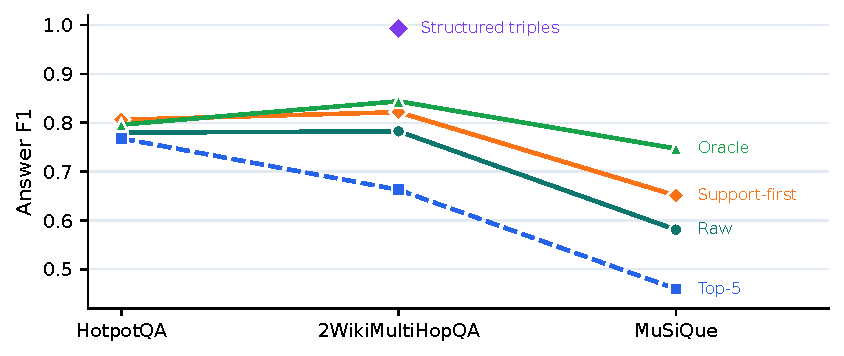
\includegraphics[width=.82\textwidth]{figs/ipm_fig1_qwen14b_interface_hierarchy.pdf}
\caption{Qwen14B rank-8 interface hierarchy at train size 4000. Oracle
support-first, oracle support, and gold structured evidence are diagnostic
upper bounds, not deployable retrieval methods. Realistic top-5 windows reduce
prompt length but do not close the gap to these oracle diagnostics.}
\label{fig:qwen14b-interface-hierarchy}
\end{figure}

\subsection{Realistic Retrieval Windows}

The realistic top-5 windows test a different question from the oracle
diagnostics. They reduce average prompt length substantially, using about 685
tokens on HotpotQA, 624 on 2WikiMultiHopQA, and 700 on MuSiQue. Their F1 scores
are 0.768, 0.663, and 0.459. These rows should not be interpreted as evidence
that top-5 retrieval is intrinsically bad. They combine two choices: which
evidence survives ranking and truncation, and how the surviving evidence is
presented to the reader.

This distinction explains why the paper treats retrieval windows in a separate
support-recall analysis. If a top-5 window lacks complete support, then the
reader has no chance to recover the correct multi-hop answer from that prompt.
If support is present, then prompt length, ordering, and distractor load become
reader-interface questions. The main comparison therefore separates diagnostic
upper bounds from realistic retrieval windows rather than treating all columns
as competing methods.

\subsection{Position and Distractor Diagnostics}

The oracle support-first diagnostic can be misunderstood as a trivial
``put evidence at the beginning'' effect. We therefore compare several
full-context HotpotQA variants that keep the same documents and roughly the
same prompt length while changing the placement of the annotated support
block. Table~\ref{tab:hotpotqa-position} reports the Qwen14B rank-8 results at
train size 2000.

\begin{table}[t]
\centering
\caption{HotpotQA full-context support-position controls with Qwen14B rank-8
at train size 2000. Dagger-marked rows use annotated support placement and are
oracle diagnostic controls, not deployable retrieval methods.}
\label{tab:hotpotqa-position}
\small
\begin{tabular}{lcc}
\toprule
Interface & Support placement & F1 \\
\midrule
Raw context & Original dataset order & 0.748 \\
\diagiface{Support shuffled} & Deterministic random block position & 0.754 \\
\diagiface{Support middle} & Support block moved to middle & 0.776 \\
\diagiface{Support last} & Support block moved to end & 0.789 \\
\diagiface{Support first} & Support block moved to front & 0.801 \\
\bottomrule
\end{tabular}
\end{table}

The result is more nuanced than a simple position story. Oracle support-first
is the strongest setting, but support-last is also substantially above raw
context. This suggests that the gain is not only from placing support near the
beginning. Grouping the support documents and moving the group to a clear
prompt boundary also helps. The middle and shuffled settings are weaker, which
is consistent with the broader long-context observation that evidence placed
inside a block of distractors can be harder to use \citep{liu2023lost}.

For the paper's main claim, Table~\ref{tab:hotpotqa-position} keeps the
evidence pool fixed. The differences come from support placement, grouping, and
distractor load, so this remains a diagnostic oracle rather than a deployable
retriever.

\section{Adaptation and Scaling Analysis}

\begin{center}
\begin{minipage}[t]{0.56\textwidth}
\centering
\sidetablecaption{tab:qwen14b-scaling-compact}{Compact Qwen14B rank-8 scaling
summary. Dagger-marked SF columns use oracle support-first as a diagnostic
control; gains are F1 differences over raw context at the same train size.}
\scriptsize
\setlength{\tabcolsep}{2.5pt}
\begin{tabular}{lccccccc}
\toprule
Dataset & Early $n$ & Raw & \diagiface{SF} & Gain & Raw (4k) & \diagiface{SF} (4k) & Gain (4k) \\
\midrule
HotpotQA & 500 & 0.727 & 0.766 & +0.039 & 0.780 & 0.806 & +0.026 \\
2Wiki & 1000 & 0.691 & 0.767 & +0.076 & 0.782 & 0.822 & +0.040 \\
MuSiQue & 1000 & 0.512 & 0.577 & +0.065 & 0.581 & 0.651 & +0.070 \\
\bottomrule
\end{tabular}
\end{minipage}
\hfill
\begin{minipage}[t]{0.40\textwidth}
\centering
\sidetablecaption{tab:restricted-adaptation-compact}{HotpotQA
restricted-adaptation diagnostic with the 1B reader at $n=500$.
Dagger-marked rows are oracle controls.}
\scriptsize
\setlength{\tabcolsep}{2.7pt}
\begin{tabular}{lcc}
\toprule
Interface & Restr. F1 & Std. F1 \\
\midrule
Raw context & 0.265 & 0.379 \\
\diagiface{Support-first} & 0.378 & 0.539 \\
\diagiface{Oracle support} & 0.527 & 0.605 \\
\bottomrule
\end{tabular}
\end{minipage}
\end{center}

\subsection{Training-Data Scaling}

The scaling question is whether raw context is mainly data-hungry. Increasing
the training set improves all evidence interfaces, but it does not make the
interface choice disappear. On HotpotQA with the 1B reader, raw context
improves from 0.379 F1 at 500 training examples to 0.554 at 4000. Oracle
support-first context also improves, from 0.539 to 0.667, and gold supporting
sentences improve from 0.605 to 0.725. The important point is not only that
more data helps. It is that the cleaner interfaces start from a higher point
and keep that advantage across the sweep.

The same pattern appears with the 3B HotpotQA reader. Raw context improves
from 0.555 F1 at 500 examples to 0.660 at 2000 examples. Oracle support-first rises
from 0.693 to 0.735 over the same range, and gold evidence improves from 0.729
to 0.769. The raw-context gap narrows with more data: oracle support-first is 0.138
F1 above raw at 500 examples and 0.075 above raw at 2000 examples. This is
useful evidence for scale, but it is not evidence that the raw interface has
caught up. Even after additional data, simply moving the support to the front
of the same context remains better than the original raw ordering.

The Qwen14B sweeps give a similar large-reader check
(Table~\ref{tab:qwen14b-scaling-compact}). On HotpotQA, the oracle
support-first gain over raw context is +0.039 F1 at 500 examples, peaks at
+0.055 at 1000 examples, and narrows to +0.026 at 4000 examples. On
2WikiMultiHopQA, the gain falls from +0.076 at 1000 examples to +0.040 at 4000
examples. On MuSiQue, the gain remains around +0.065--+0.070. Larger readers
and larger training sets therefore reduce some interface gaps, especially on
the easier or shorter settings, but they do not remove the interface gap.
Appendix~\ref{app:full-interface-results} reports the full Qwen14B scaling
rows and the cross-reader support-first gains behind this compact summary.

\subsection{Adaptation-Capacity Analysis}

The restricted-adaptation runs ask the same question under a tighter update
budget. The goal is not to estimate a formal intrinsic dimension for each
interface. The goal is simpler: under the same constrained update budget, does
one evidence form remain easier for the reader to adapt to than another?

The HotpotQA hash-projection sweep gives the clearest check. With the 1B
reader, rank-8 adapters, 500 training examples, and 262,144 active projected
dimensions, raw context reaches 0.265 F1. Oracle support-first context reaches 0.378
F1 under the same constraint, and gold supporting sentences reach 0.527 F1.
Table~\ref{tab:restricted-adaptation-compact} places the restricted runs next
to the matched standard rank-8 references. The point is not the absolute gap to
the reference. The point is that the same constrained update budget preserves
the same interface ordering: raw context is hardest, oracle support-first is easier,
and clean support is easiest.

This result should be interpreted as supporting evidence, not as the central
claim of the paper. The main object is still the evidence interface. LoRA rank
and restricted subspaces are useful because they make adaptation burden visible
under controlled budgets.

\subsection{Frozen-Reader Sanity Check}

A separate sanity check asks whether the broad interface ordering is visible
even without LoRA adaptation. Table~\ref{tab:frozen-qwen14b-sanity} evaluates
the frozen Qwen14B reader on 300 HotpotQA validation examples. This is not a
full zero-shot benchmark and is not used as the main result, but it rules out
the narrow explanation that the interface gap appears only after supervised
reader adaptation.

\begin{table}[!t]
\centering
\caption{Frozen Qwen14B HotpotQA anchor with 300 validation examples. The
reader is not LoRA-adapted. The dagger-marked row uses annotated support and is
an oracle diagnostic, not a deployable retrieval method.}
\label{tab:frozen-qwen14b-sanity}
\small
\setlength{\tabcolsep}{4pt}
\begin{tabular}{lrrrr}
\toprule
Interface & EM & F1 & Ans. cont. & Avg tokens \\
\midrule
No context & 0.143 & 0.219 & 0.193 & 61 \\
Raw context & 0.460 & 0.630 & 0.603 & 1484 \\
FT cross-enc top-5 & 0.477 & 0.626 & 0.617 & 685 \\
\diagiface{Oracle support} & 0.557 & 0.738 & 0.663 & 156 \\
\bottomrule
\end{tabular}
\end{table}

The frozen reader still benefits strongly from external evidence: raw context
is 0.411 F1 above question-only input. The compact oracle-support diagnostic is
another 0.108 F1 above raw context while using far fewer tokens. The realistic
top-5 window is close to raw context in this HotpotQA anchor, consistent with
the high support recall reported later. The sanity check therefore supports
the same interpretation as the adapted-reader experiments: evidence must be
available, but the reader-facing form also changes how useful that evidence is.

\subsection{Model-Family and Model-Size Scaling}

Table~\ref{tab:support-first-cross-reader-summary} and
Figure~\ref{fig:support-first-gain} summarize the matched oracle support-first
gain over raw context across the evaluated reader families. Each point in the
figure compares raw context and oracle support-first context for the same
dataset, reader, train size, LoRA rank, and prompt length. Across the 19
conditions in the plot, the gain is positive in every completed matched
condition.

The gains are not uniform across datasets. HotpotQA shows the smallest but
still positive gains, ranging from 0.014 to 0.081 F1 with a mean of 0.046.
2WikiMultiHopQA ranges from 0.032 to 0.115 with a mean of 0.075. MuSiQue has
the largest gains, from 0.070 to 0.159 with a mean of 0.109. This ordering is
consistent with the interface interpretation: the longer and more
composition-heavy MuSiQue contexts impose a larger evidence-organization
burden, so the oracle support-first diagnostic has more room to help.
Appendix~\ref{app:full-interface-results} reports the per-reader rows behind
the compact summary.

The cross-model result also guards against a narrow model-family explanation.
The oracle support-first gain appears for 1B and 3B Llama readers, several 7B--9B
readers, and the Qwen14B anchor. Larger models often reduce the gap, but they
do not erase it in these matched conditions. This comparison is deliberately
within-reader: a point is included only when raw context and oracle
support-first share the same dataset, model, training size, and adaptation
budget. The positive direction therefore cannot be attributed to swapping in a
larger reader or an easier split. The practical implication is that evidence
organization should be evaluated as a reader-interface design choice, not only
as a weakness of small models. The figure is therefore not a model leaderboard;
its role is to check whether the same interface contrast survives across
reader families and dataset formats under matched supervision.

\begin{center}
\sidetablecaption{tab:support-first-cross-reader-summary}{Cross-reader oracle
support-first gain summary. Gains are F1 differences over raw context in
matched reader--dataset conditions.}
\scriptsize
\setlength{\tabcolsep}{6pt}
\begin{tabular}{lcccc}
\toprule
Dataset & Readers & Mean gain & Gain range & Positive \\
\midrule
HotpotQA & 6 & +0.046 & [+0.014, +0.081] & 6/6 \\
2WikiMultiHopQA & 7 & +0.075 & [+0.032, +0.115] & 7/7 \\
MuSiQue & 6 & +0.109 & [+0.070, +0.159] & 6/6 \\
\bottomrule
\end{tabular}
\end{center}

\begin{figure}[!h]
\centering
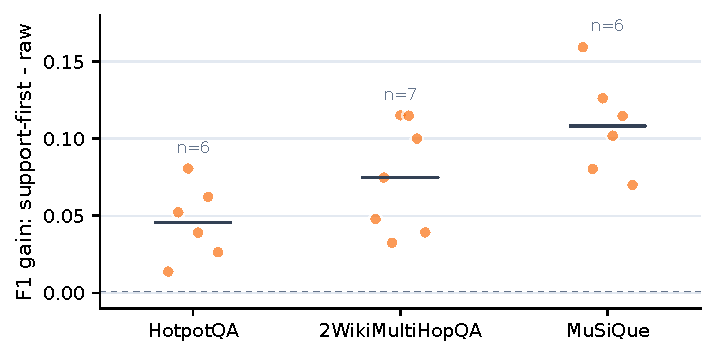
\includegraphics[width=.68\textwidth]{figs/ipm_fig2_support_first_gain.pdf}
\caption{Oracle support-first diagnostic gain over raw context across available
reader families. Each point is one matched model--dataset condition, and the
black segment marks the dataset median. The MuSiQue Gemma-2-9B condition is
omitted because its matched raw-context counterpart is not available. The plot
summarizes matched interface contrasts rather than ranking model families, so
it should be read as directionality evidence rather than a full model-size
benchmark.}
\label{fig:support-first-gain}
\end{figure}
\FloatBarrier

\section{Retrieval Quality, Cost, and Reader Usability}

\subsection{Realistic Retrieval Windows}

Realistic retrieval windows are deployable prompt-budget interfaces. They can
help by removing distractors and shortening the prompt, but they can also hurt
by dropping one of the support units needed for a multi-hop answer. For that
reason, we evaluate each top-$k$ window with both downstream F1 and
complete-support recall, where complete support means that every annotated
support document or paragraph survives truncation.

Table~\ref{tab:retrieval-recall-cost} joins the Qwen14B main results with
validation support recall for the corresponding top-5 retrieval window.
The HotpotQA window uses the fine-tuned cross-encoder because it is the
strongest realistic HotpotQA retriever in our pool. The 2WikiMultiHopQA
and MuSiQue windows use the off-the-shelf cross-encoder. The table should be
read as a cost--coverage--quality tradeoff rather than as a pure answer-quality
comparison.
Appendix~\ref{app:retrieval-support-recall} gives the full support-recall table
for BM25, cross-encoder, and fine-tuned cross-encoder windows.
Appendix~\ref{app:full-interface-results} also reports order-only and top-$k$
controls, which separate ranking-induced ordering changes from truncation.

\begin{table}[t]
\centering
\caption{Support recall, answer quality, and prompt cost for Qwen14B retrieval
windows at train size 4000. All-support recall measures whether all
gold-annotated support units appear in the window; F1 $\Delta$ is top-5 minus
raw context.}
\label{tab:retrieval-recall-cost}
\small
\setlength{\tabcolsep}{2.8pt}
\begin{tabular}{lcccccc}
\toprule
Dataset & Supp.@5 & Supp.@10 & Raw F1 & Top-5 F1 & F1 $\Delta$ & Token red. \\
\midrule
HotpotQA & 0.948 & 1.000 & 0.780 & 0.768 & $-0.012$ & 53.8\% \\
2WikiMultiHopQA & 0.597 & 1.000 & 0.782 & 0.663 & $-0.120$ & 41.1\% \\
MuSiQue & 0.313 & 0.527 & 0.581 & 0.459 & $-0.121$ & 71.7\% \\
\bottomrule
\end{tabular}
\end{table}

The three datasets occupy different regimes. HotpotQA is the favorable case
for retrieval windowing. The fine-tuned cross-encoder top-5 window contains all
support documents for 94.8\% of validation examples, cuts the prompt by 53.8\%,
and loses only 0.012 F1 relative to raw context. Here the support chain is
usually still present, so the top-5 window mostly acts as a cost-saving
interface. The small F1 loss should be interpreted as the residual price of
truncation and presentation, not as a major retrieval failure.

2WikiMultiHopQA is a mixed case. The top-5 window reduces prompt length by
41.1\%, but complete-support recall is only 59.7\%. Because support@10 reaches
1.000, this loss is largely a top-5 coverage problem rather than evidence that
the reader cannot use retrieved evidence. In many examples, the window is
missing at least one required hop. A reader-side interface cannot recover a
relation chain that is not present in the input.

MuSiQue is the clearest coverage-limited case. The top-5 window cuts tokens by
71.7\%, but contains all support paragraphs for only 31.3\% of validation
examples and loses 0.121 F1 relative to raw context. Even support@10 is only
0.527, so this is not just an overly tight top-5 setting. For this dataset, the
first fix is higher support coverage through a better retriever, a larger
window, or a selection objective that is aware of multi-hop coverage, as in
retrieval-and-reasoning approaches for multi-step QA
\citep{asai2020reasoningpaths,trivedi2023ircot}.

\subsection{Support Recall versus Answer Quality}
\label{sec:support-recall}

The recall results explain why full-context reordering and top-$k$ truncation
should not be merged into one conclusion. A full ordered context keeps the
candidate pool fixed and changes where the support appears. That is why the
oracle support-first diagnostic can be interpreted as a reader-usability probe.
A top-$k$ window changes both the amount of text and the evidence available to
the reader. Its F1 therefore combines retrieval coverage, prompt cost, and
reader usability.

This distinction changes how we interpret failures. If complete-support recall
is high and F1 is still low, the reader or the presentation of evidence is a
plausible bottleneck. If complete-support recall is low, the main bottleneck is
earlier: the selected window does not contain the full support chain. In our
main top-5 results, HotpotQA is close to the first regime, while MuSiQue is
firmly in the second. 2WikiMultiHopQA falls between them.

A per-example split confirms this interpretation. Among examples where the
top-5 window contains complete support, top-5 is tied with raw context on
HotpotQA ($+0.000$ F1), nearly tied on 2WikiMultiHopQA ($-0.006$), and higher
on MuSiQue ($+0.088$). Among examples where top-5 misses at least one support
unit, the corresponding drops are much larger: $-0.223$, $-0.273$, and
$-0.236$ F1. The negative top-5 averages in
Table~\ref{tab:retrieval-recall-cost} are therefore mostly coverage failures
on the harder datasets, not evidence that shorter reader-facing windows are
always worse.

The practical rule is therefore sequential. Retrieval must first preserve
enough support. Once evidence availability is high, interface design can focus
on making the support easier for the reader to use through ordering, grouping,
shortening, or structured presentation. Interface analysis does not replace
retrieval evaluation; it adds a second measurement axis after evidence
availability is checked.

\begin{figure}[!t]
\centering
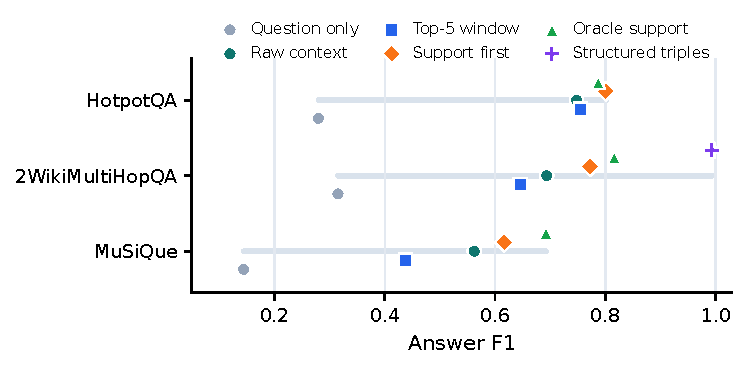
\includegraphics[width=.80\textwidth]{figs/ipm_fig3_no_context_gap.pdf}
\caption{Qwen14B rank-8 no-context gap at train size 2000. Points show
question-only adaptation and evidence-bearing interfaces for each dataset; the
gray segment marks the span from question-only to the strongest shown evidence
interface.}
\label{fig:no-context-gap}
\end{figure}

\subsection{Ranker and Window Controls}

The top-5 results above are not meant to depend on one arbitrary ranker or one
unexamined window. The full controls in
Appendix~\ref{app:full-interface-results} compare ranker-induced full-context
ordering and top-$k$ truncation at the Qwen14B train-size-2000 setting. These
controls show why we separate ordering from support coverage. When the full
evidence pool is kept and only the order changes, HotpotQA raw context rises
from 0.748 F1 to 0.761 under BM25 order, while 2WikiMultiHopQA rises from
0.694 to 0.736 under cross-encoder order. MuSiQue moves in the opposite
direction: raw context is 0.562, while BM25 and cross-encoder full-order
variants fall to 0.539 and 0.522. Ordering alone can help, but it is not a
universal fix.

The truncation controls show the other side of the tradeoff. On HotpotQA, the
fine-tuned cross-encoder top-5 window reaches 0.755 F1 at about 685 tokens,
well above BM25 top-5 (0.690) and the off-the-shelf cross-encoder top-5
(0.674). On 2WikiMultiHopQA, cross-encoder top-5 is slightly above BM25 top-5
(0.646 versus 0.629). On MuSiQue, cross-encoder top-5 improves over BM25
top-5 (0.437 versus 0.377) but remains far below raw context, matching the
support-recall finding that many MuSiQue windows simply miss required support.
Thus the retrieval-window result is not a single cherry-picked comparison: it
reflects a recurring cost--coverage tradeoff that varies by dataset.

\begin{center}
\sidetablecaption{tab:ranker-window-compact}{Compact ranker and truncation
controls with Qwen14B rank-8 readers at train size 2000. Full-order rows keep
the evidence pool fixed; top-5 rows truncate to a retrieval window.}
\scriptsize
\setlength{\tabcolsep}{4pt}
\begin{tabular}{lccccc}
\toprule
Dataset & Raw F1 & Best full-order F1 & Full-order $\Delta$ & Best top-5 F1 & Top-5 $\Delta$ \\
\midrule
HotpotQA & 0.748 & 0.761 (BM25) & +0.013 & 0.755 (FT CE) & +0.007 \\
2WikiMultiHopQA & 0.694 & 0.736 (CE) & +0.042 & 0.646 (CE) & $-0.048$ \\
MuSiQue & 0.562 & 0.539 (BM25) & $-0.023$ & 0.437 (CE) & $-0.125$ \\
\bottomrule
\end{tabular}
\end{center}

\subsection{Prompt-Token Cost versus Accuracy}

Prompt cost changes the system-level interpretation of the same answer score,
which is also why prompt-compression and reader-aware reranking methods report
cost together with answer behavior \citep{jiang2023longllmlingua,yu2024rankrag}.
The top-5 windows in Table~\ref{tab:retrieval-recall-cost} reduce average
prompt length by 41--72\%, so a small F1 loss may be acceptable when support
recall is high. The HotpotQA result is closest to this operating point: the
window saves more than half the prompt tokens while preserving nearly all
support chains. The MuSiQue result is not: the token saving is large, but most
examples lose at least one support paragraph. The same token reduction can
therefore be either a useful efficiency gain or a harmful evidence-coverage
loss, depending on recall.

Figure~\ref{fig:no-context-gap} gives a complementary large-reader view of how
much context matters relative to question-only adaptation. Across datasets,
question-only adaptation remains far below the evidence-bearing interfaces.
The no-context gap is useful because it rules out a trivial explanation that
the reader is mostly answering from parametric memory or dataset priors. The
retrieval and oracle interfaces matter because they supply external evidence,
but their utility depends on two conditions: the evidence must be present, and
it must be organized in a form the reader can use. Section~8 tests the first
condition more directly by removing support from evidence-bearing prompts.

\section{Evidence Reliance and Robustness}

\subsection{Answer-Likelihood and Context Utility}

Answer F1 measures the final generated string, but it does not directly show
whether the reader's probability of the gold answer depends on the supplied
evidence. We therefore run an additional HotpotQA diagnostic with the 3B
rank-8 readers at train size 2000. For each trained interface, we measure
answer negative log-likelihood (NLL) under the original evidence interface,
under a question-only input, and under a no-support ablation that removes the
annotated supporting documents from the evidence field.

Table~\ref{tab:hotpotqa-reliance} reports the compact version of this
diagnostic. In this HotpotQA setting, all original evidence-bearing interfaces
have much lower answer NLL than the question-only input. The ordering is also consistent with the
main F1 results: oracle support has the lowest answer NLL, followed by
oracle support-first, raw context, and the fine-tuned top-5 window. This gives a
likelihood-side check that the interface gap is not only a decoding artifact.
Appendix~\ref{app:error-cases} reports the expanded reliance table together
with fine-grained error tags and representative paired examples.

\subsection{Support Removal and Position Stress Tests}

The no-support ablation gives the stronger reliance check. Removing the
supporting documents pushes answer NLL back near or above the question-only
range and collapses generation F1. For example, the oracle support-first reader drops
from 0.738 F1 to 0.168 F1 after support removal, and the fine-tuned top-5
reader drops from 0.714 to 0.196. For the same four readers, question-only F1
falls in the narrow range 0.245--0.258, so the no-support generations are back
near the no-context regime. The evidence-bearing gains are therefore not just
format effects: they depend on the presence of the supporting documents.

Together with the position controls in
Table~\ref{tab:hotpotqa-position}, this separates two properties. Removing
support tests whether the reader relies on the evidence at all. Reordering the
same full context tests whether the reader can use the evidence when it is
present but buried or split among distractors. Both diagnostics point in the
same direction: evidence availability is necessary, but organization changes
how usable that evidence is.

\begin{table}[t]
\centering
\begin{minipage}[t]{0.55\textwidth}
\centering
\sidetablecaption{tab:hotpotqa-reliance}{HotpotQA evidence reliance.
Dagger-marked rows use gold support annotations and are oracle diagnostic
controls.}
\scriptsize
\setlength{\tabcolsep}{2.4pt}
\begin{tabular}{lcccc}
\toprule
Interface & Orig. NLL & No-supp. NLL & Orig. F1 & No-supp. F1 \\
\midrule
Raw context & 0.443 & 2.468 & 0.656 & 0.227 \\
\diagiface{Support-first} & 0.413 & 3.052 & 0.738 & 0.168 \\
\diagiface{Oracle support} & 0.356 & 2.049 & 0.764 & 0.241 \\
FT top-5 & 0.516 & 2.527 & 0.714 & 0.196 \\
\bottomrule
\end{tabular}
\end{minipage}
\hfill
\begin{minipage}[t]{0.42\textwidth}
\centering
\sidetablecaption{tab:error-taxonomy}{High-contrast oracle support-first
diagnostic win-case taxonomy. Cases are selected by a strict paired threshold
and tagged by deterministic rules.}
\scriptsize
\setlength{\tabcolsep}{2.6pt}
\begin{tabular}{lcccc}
\toprule
Dataset & Cases & Layout & Entity/hop & Other \\
\midrule
HotpotQA & 7 & 4 & 1 & 2 \\
2Wiki & 17 & 10 & 5 & 2 \\
MuSiQue & 18 & 14 & 4 & 0 \\
\bottomrule
\end{tabular}
\end{minipage}
\end{table}

\subsection{Error Analysis}

Finally, we inspect paired Qwen14B train-size-4000 cases where raw context
fails while the oracle support-first diagnostic succeeds. We count a case when
raw-context F1 is at most 0.2 and oracle support-first F1 is at least 0.8 on the same
validation example. This yields 7 HotpotQA cases, 17 2WikiMultiHopQA cases, and
18 MuSiQue cases among the 300 evaluated examples per dataset, or 2.3\%,
5.7\%, and 6.0\% of each evaluated subset. These are high-contrast failures
where reorganization helps, not a representative sample of all mistakes. The
tags in Table~\ref{tab:error-taxonomy} are rule-based diagnostic labels derived
from the raw prediction, support positions, and dataset metadata; they are
meant to guide inspection rather than replace a final human annotation study.
Appendix~\ref{app:error-cases} gives the full tag breakdown behind the compact
taxonomy, while Table~\ref{tab:error-examples} gives representative paired
examples.

Within this high-contrast subset, the largest rule-based category is layout:
the supporting documents are late in the raw context or split by distractors.
This accounts for 4 of 7 HotpotQA win cases, 10 of 17 2WikiMultiHopQA cases,
and 14 of 18 MuSiQue cases. The second category is entity or hop confusion,
where the raw-context reader returns a nearby entity, a distractor entity, or
an intermediate-hop answer. For example, in one MuSiQue case the raw reader
answers with an intermediate location near Wenzhou, while oracle support-first returns
the required county. In a 2Wiki comparison case, raw context chooses the wrong
film from the pair, while oracle support-first chooses the earlier film.

These examples make the interface bottleneck concrete. The support is not
missing from the raw context; the reader is seeing it in a harder layout. When
the same support is grouped and moved to a clear prompt boundary, many of these
errors disappear. The tags are conservative because they count only clear
high-contrast wins, not partial improvements where both interfaces remain
partly wrong. Because each pair keeps the question, answer target, and evidence
pool fixed, these cases isolate presentation failures more cleanly than an
aggregate error count. These are not retrieval-miss examples; the needed support
is present but harder to use. This is the operational reason to distinguish
evidence retrieval from evidence interface design.

\begin{table}[!b]
\centering
\caption{Representative raw-context failures fixed by oracle support-first.
Cases are selected from high-contrast paired wins where raw-context F1 is at
most 0.2 and oracle support-first F1 is at least 0.8.}
\label{tab:error-examples}
\scriptsize
\setlength{\tabcolsep}{3pt}
\begin{tabular}{p{0.14\textwidth}p{0.28\textwidth}p{0.14\textwidth}p{0.17\textwidth}p{0.17\textwidth}}
\toprule
Dataset & Question cue & Gold & Raw prediction & Oracle SF prediction \\
\midrule
HotpotQA & Lead character in \emph{Get Smart} & Maxwell Smart & Agent 99 & Maxwell Smart \\
HotpotQA & John Moncur's Ipswich Town league & Championship & Premier League & Championship \\
2WikiMultiHopQA & Director of \emph{A Winter of Cyclists} born where & Irish & Munster & Irish \\
2WikiMultiHopQA & Which film came out earlier & Khote Sikkey & Moscow Chill & Khote Sikkey \\
MuSiQue & Zhejiang place where Protestants are notable & Yongjia County & near Wenzhou & Yongjia County \\
MuSiQue & NBA draft pick before top scoring-season player & Greg Oden & Markelle Fultz & Greg Oden \\
\bottomrule
\end{tabular}
\end{table}

\section{Discussion}

\subsection{Retriever--Reader Interfaces}

The main implication is that a RAG system should treat the reader input as a
design choice, not as a direct dump of retriever output. Retrieval produces a
candidate evidence pool; the interface still decides which units are shown,
where they appear, how much distractor text remains, and whether evidence is
kept as raw text or made more compact. In our matched comparisons, these
choices change answer quality even when the reader family, answer target,
training size, and LoRA rank are fixed.

This is a reader-side design problem as well as a retrieval problem. A short
top-$k$ window can save tokens and still fail if it drops one required hop. A
full context can contain the support and still be difficult when the evidence
is late, split, or surrounded by distractors. The oracle support-first
diagnostic exposes this interface gap by keeping the evidence pool roughly
fixed while changing its organization. The realistic retrieval-window results
show the complementary failure mode: prompt compression helps only after
support coverage is high enough.

\subsection{Diagnostics versus Deployment}

The oracle interfaces are measurement tools, not production methods. Oracle
support-first and oracle support require gold support annotations, and the
2Wiki structured triples require a gold reasoning chain. They estimate what is
lost when evidence is present but poorly organized, or what is possible when
support is clean and compact. They do not solve evidence selection.

The deployable-style interfaces in this paper are the retrieval and reranking
windows. They ask how much of the diagnostic gap can be closed by practical
ranking under a prompt budget. HotpotQA is the favorable case: support recall
is high, token cost drops by more than half, and F1 changes little.
2WikiMultiHopQA and MuSiQue are cautionary: when support recall is low,
truncation becomes a coverage failure before it can be judged as a
reader-interface design.

\subsection{Guidance and Limits}

The practical order is simple. First, measure complete-support recall for the
selected window. In our results, support@5 near 0.95 on HotpotQA behaves like
useful compression, support@5 near 0.6 on 2WikiMultiHopQA is a mixed regime,
and support@5 near 0.3 on MuSiQue is coverage-limited. These are not universal
thresholds, but they give a validation check: if the window often drops a
required hop, improve retrieval coverage before tuning reader formatting.
Table~\ref{tab:coverage-regimes} extracts the corresponding recall regimes
from the full appendix table. Second, once coverage is high, optimize the
reader-facing form through support grouping, stable boundaries, compact
summaries, or reranking objectives that reward usable evidence. Third, use
structured evidence only when trustworthy structure is available; the 2Wiki
triple result is an upper bound on compact relational evidence, not evidence
that arbitrary passages should be converted into triples.

\begin{table}[!t]
\centering
\caption{Support-coverage regimes behind the practical guidance. All@k is
complete-support recall: every annotated support unit survives the retrieval
window.}
\label{tab:coverage-regimes}
\scriptsize
\setlength{\tabcolsep}{5pt}
\begin{tabular}{llccc}
\toprule
Dataset & Ranker & All@5 & All@10 & Latest support rank \\
\midrule
HotpotQA & FT cross-encoder & 0.948 & 1.000 & 2.63 \\
2WikiMultiHopQA & Cross-encoder & 0.597 & 1.000 & 4.88 \\
MuSiQue & Cross-encoder & 0.313 & 0.527 & 10.54 \\
\bottomrule
\end{tabular}
\end{table}

\subsection{Limitations and Future Work}

The study is intentionally bounded to multi-hop QA, where evidence organization
is visible because answers require multiple support units. Single-hop QA,
dialogue, and longer document collections may show different tradeoffs. The
largest reader is Qwen14B; larger 20B--30B readers remain useful scale checks,
although the current cross-model pattern already rules out a single-small-model
artifact. The main experiments use LoRA-adapted readers and fixed 300-example validation
subsets so that many matched interface, model, training-size, and retrieval
variants can be compared. These controls make interface effects measurable,
but they do not replace full held-out benchmark evaluation, repeated subset
sampling, or broader zero-shot and few-shot reader studies. A second boundary is evaluation granularity. The fixed subsets make paired
comparisons affordable and keep the question set identical across interfaces,
which is important for isolating interface effects. They are not meant to
replace full benchmark reporting. The paired bootstrap intervals reduce the
risk that the main deltas are single-sample artifacts, while future versions
should repeat subset sampling and run larger held-out splits for the most
important interfaces. The oracle structured and error-taxonomy analyses are also diagnostic. The
2Wiki triples use dataset-provided gold reasoning structure, and the error tags
are rule-based labels for finding recurring failure modes. These limitations
mainly constrain how far the results should be generalized, not the matched
within-reader contrasts reported here. Future work should test learned selectors
or compressors that preserve support coverage, control prompt cost, and present
evidence in forms that readers can use reliably.

\section{Conclusion}

This paper studies evidence interfaces for retrieval-augmented question
answering: the form in which retrieved or oracle evidence is shown to the
reader. Across HotpotQA, 2WikiMultiHopQA, and MuSiQue, the same reader can
behave differently when the same evidence is raw, oracle-reordered, truncated
by a retriever, or converted into compact structured evidence. The main claim
is narrow but practical. Retrieval relevance is necessary, but it is not the
whole RAG interface: evidence also needs to survive the selected window and be
organized in a form the reader can use. The experiments show why these two
requirements should be reported together. A top-$k$ window can be useful
compression when complete support survives, but the same token saving becomes
a coverage failure when one required hop is dropped. The no-support and paired
error diagnostics then test the reader side of the handoff: whether the model
actually relies on the supporting evidence and where raw context makes that
evidence harder to use. This framing also prevents a common misreading of the
oracle rows. They are not proposed production systems; they are probes for
estimating how much quality is lost between evidence availability and evidence
use. Future RAG pipelines should therefore evaluate the retriever--reader
handoff directly, including support coverage, ordering, prompt cost, and
structure before generation. The useful optimization target is not only a
ranked document list, but the reader input produced from that list. The
deployable next step is to close that gap with rankers, compressors, or
structure extractors that preserve complete support while producing shorter and
cleaner reader inputs.

\section*{Data Availability}

An anonymized artifact will be made available during review. The artifact will
include code, configuration files, prompt templates, aggregate result tables,
and plotting scripts needed to reproduce the reported analyses. The experiments
use public third-party datasets and model checkpoints, which should be obtained
from their original providers under their respective licenses. The artifact
will not include credentials, local machine paths, private logs,
non-redistributable model checkpoints, or raw third-party dataset copies. When
redistribution is restricted, released files will contain derived aggregate
tables and reconstruction scripts rather than the original dataset text; users
should rebuild those artifacts from locally obtained dataset copies. The
archive will also map released tables and figures to the corresponding
manuscript results so that reported numbers can be traced without private logs.

\clearpage
\bibliographystyle{model1-num-names}
\bibliography{cas-refs}

\clearpage
\appendix
\renewcommand{\arraystretch}{0.88}
\setcounter{table}{0}
\setcounter{figure}{0}
\setcounter{equation}{0}
\makeatletter
\@addtoreset{table}{section}
\@addtoreset{figure}{section}
\@addtoreset{equation}{section}
\makeatother
\renewcommand{\thetable}{\Alph{section}.\arabic{table}}
\renewcommand{\thefigure}{\Alph{section}.\arabic{figure}}
\renewcommand{\theequation}{\Alph{section}.\arabic{equation}}

\section{Interface Construction Details}
\label{app:interface-construction}

This appendix gives the concrete construction rules. Oracle support-first,
oracle support, position controls, and structured triples use gold support
fields or gold structure; retrieval windows use ranker outputs.
The purpose is to make the interface definitions behind
Table~\ref{tab:interface-families} precise enough to audit. These construction
rules also explain why the paper separates deployable retrieval windows from
oracle diagnostics in Table~\ref{tab:qwen14b-main-scaling}: some interfaces can
be built from ordinary ranked evidence, while others require gold support
annotations and should be read only as measurement probes.

\paragraph{Raw context.}
The raw interface keeps the dataset-provided context order or the full ranked
order for retrieval-derived variants.

\paragraph{Oracle support-first.}
The support-first diagnostic extracts annotated support units in dataset order,
then appends non-support units in their original order.

\paragraph{Position controls.}
The HotpotQA position controls use the same support and non-support units, but
place the support block at the front, middle, end, or a deterministic shuffled
position.

\paragraph{Oracle support and structured evidence.}
Oracle support keeps only annotated supporting sentences or paragraphs.
For 2WikiMultiHopQA, the structured interface converts the gold reasoning chain
into compact relation-style triples.

\paragraph{Retrieval windows.}
Top-$k$ windows select the highest-ranked units from BM25, a cross-encoder, or a
fine-tuned cross-encoder. Ordered full-context variants keep the evidence pool
but sort it by the ranker; truncated windows keep only the top $k$ units.

\begin{center}
\sidetablecaption{tab:appendix-dataset-units}{Dataset-specific evidence units
and gold fields used to construct the interfaces.}
\scriptsize
\setlength{\tabcolsep}{3.2pt}
\begin{tabular}{>{\raggedright\arraybackslash}p{0.18\textwidth}
                >{\raggedright\arraybackslash}p{0.25\textwidth}
                >{\raggedright\arraybackslash}p{0.30\textwidth}
                >{\raggedright\arraybackslash}p{0.18\textwidth}}
\toprule
Dataset & Raw evidence pool & Annotated support field & Structured field \\
\midrule
HotpotQA & Distractor paragraphs with support labels &
Supporting-fact titles/sentences & None \\
2WikiMultiHopQA & Candidate articles with support sentences &
Supporting titles/sentences & Gold reasoning triples \\
MuSiQue & Candidate paragraphs &
Supporting paragraphs & None \\
\bottomrule
\end{tabular}
\end{center}

Table~\ref{tab:appendix-dataset-units} explains why the same interface name can
correspond to different evidence units across datasets. HotpotQA exposes
sentence-level supporting facts inside paragraphs, 2WikiMultiHopQA additionally
provides reasoning triples, and MuSiQue marks supporting paragraphs. The main
experiments therefore compare interfaces within each dataset first, and use
cross-dataset comparisons to study trends rather than to claim identical support
granularity.

This distinction matters for interpreting the oracle rows. Oracle support on
HotpotQA and 2WikiMultiHopQA is closer to sentence-level filtering, whereas
MuSiQue oracle support keeps supporting paragraphs and can still contain more
local context. The structured 2WikiMultiHopQA row is even more privileged: it
uses a dataset-provided reasoning object, not an extracted graph. For that
reason, the structured result is useful as an upper-bound diagnostic, but it
should not be compared directly to a deployable top-$k$ retrieval window. The
main text uses these rows to estimate interface headroom, not to propose that a
production RAG system has access to gold support labels.

\section{Full Interface and Scaling Tables}
\label{app:full-interface-results}

This appendix keeps the fuller numerical view. Values are validation exact
match (EM), token-level F1, answer-contained rate, or average prompt-token
count as indicated.
The tables expand the compact main-text results without changing the
interpretation: oracle rows are diagnostic upper bounds, while retrieval rows
are realistic prompt-window interfaces.
The appendix is organized to mirror the claims in the main text. First,
Table~\ref{tab:appendix-qwen14b-scaling} expands the Qwen14B scaling summary
behind Table~\ref{tab:qwen14b-scaling-compact}. Second,
Table~\ref{tab:appendix-support-first-gain} gives the per-reader values behind
Figure~\ref{fig:support-first-gain}. Third, the remaining tables separate
diagnostic controls, full-context ordering, and top-$k$ truncation so that the
retrieval-window results in Table~\ref{tab:retrieval-recall-cost} are not read
as a single isolated comparison.

\begin{table}[!hbp]
\centering
\caption{Qwen14B rank-8 training-size scaling by dataset and interface. Entries
are F1. Missing cells indicate runs not used in the current Qwen14B matrix.}
\label{tab:appendix-qwen14b-scaling}
\scriptsize
\setlength{\tabcolsep}{3.5pt}
\begin{tabular}{llcccc}
\toprule
Dataset & Interface & $n=500$ & $n=1000$ & $n=2000$ & $n=4000$ \\
\midrule
HotpotQA & Raw context & 0.727 & 0.730 & 0.748 & 0.780 \\
HotpotQA & \emph{Support first (oracle)} & 0.766 & 0.785 & 0.801 & 0.806 \\
HotpotQA & FT cross-enc top-5 & 0.742 & 0.746 & 0.755 & 0.768 \\
HotpotQA & \emph{Oracle support} & 0.761 & 0.781 & 0.787 & 0.796 \\
\midrule
2WikiMultiHopQA & Raw context & -- & 0.691 & 0.694 & 0.782 \\
2WikiMultiHopQA & \emph{Support first (oracle)} & -- & 0.767 & 0.772 & 0.822 \\
2WikiMultiHopQA & Cross-enc top-5 & -- & 0.605 & 0.646 & 0.663 \\
2WikiMultiHopQA & \emph{Oracle support} & -- & 0.789 & 0.816 & 0.844 \\
2WikiMultiHopQA & \emph{Structured triples (gold)} & -- & 0.993 & 0.993 & 0.993 \\
\midrule
MuSiQue & Raw context & -- & 0.512 & 0.562 & 0.581 \\
MuSiQue & \emph{Support first (oracle)} & -- & 0.577 & 0.617 & 0.651 \\
MuSiQue & Cross-enc top-5 & -- & 0.422 & 0.437 & 0.459 \\
MuSiQue & \emph{Oracle support} & -- & 0.689 & 0.692 & 0.747 \\
\bottomrule
\end{tabular}
\end{table}

Table~\ref{tab:appendix-qwen14b-scaling} shows that the main pattern is not an
artifact of the final 4000-example checkpoint. Raw context improves with more
training data, but oracle support-first and oracle support remain competitive or
better across the reported Qwen14B sweep. The gap narrows on some datasets and
persists on others, which is why the main text treats training scale as a
moderator rather than as a complete explanation.

The rows also separate two kinds of improvement. On HotpotQA, the deployable
fine-tuned top-5 window stays close to raw context throughout the sweep, which
is consistent with the high complete-support recall reported in
Table~\ref{tab:retrieval-recall-cost}. On 2WikiMultiHopQA and MuSiQue, the
same top-5 format remains below raw context even as the reader sees more
training examples. Those losses should be read together with
Table~\ref{tab:appendix-support-recall}: they are partly coverage failures,
not simply failures of the reader architecture. The oracle rows show the
opposite diagnostic condition: when support is known and either moved forward
or filtered, the reader generally improves, so the remaining gap is tied to
how evidence is presented rather than to answer memorization alone.

\begin{table}[!hbp]
\centering
\caption{Oracle support-first gain over raw context across available reader
families. The two interfaces use the same prompt-token budget within each row.}
\label{tab:appendix-support-first-gain}
\scriptsize
\setlength{\tabcolsep}{3.8pt}
\begin{tabular}{llrrrr}
\toprule
Dataset & Reader & Train size & Raw F1 & Oracle SF F1 & Gain \\
\midrule
HotpotQA & Llama-3.2-3B & 4000 & 0.719 & 0.733 & +0.014 \\
HotpotQA & Qwen2.5-Coder-7B & 1000 & 0.696 & 0.748 & +0.052 \\
HotpotQA & Mistral-7B & 1000 & 0.684 & 0.765 & +0.081 \\
HotpotQA & Llama-3.1-8B & 1000 & 0.721 & 0.760 & +0.039 \\
HotpotQA & Gemma-2-9B & 1000 & 0.713 & 0.776 & +0.062 \\
HotpotQA & Qwen2.5-Coder-14B & 4000 & 0.780 & 0.806 & +0.026 \\
\midrule
2WikiMultiHopQA & Llama-3.2-1B & 4000 & 0.475 & 0.523 & +0.048 \\
2WikiMultiHopQA & Llama-3.2-3B & 4000 & 0.657 & 0.732 & +0.075 \\
2WikiMultiHopQA & Qwen2.5-Coder-7B & 1000 & 0.618 & 0.650 & +0.032 \\
2WikiMultiHopQA & Mistral-7B & 1000 & 0.585 & 0.700 & +0.115 \\
2WikiMultiHopQA & Llama-3.1-8B & 1000 & 0.582 & 0.697 & +0.115 \\
2WikiMultiHopQA & Gemma-2-9B & 1000 & 0.665 & 0.765 & +0.100 \\
2WikiMultiHopQA & Qwen2.5-Coder-14B & 4000 & 0.782 & 0.822 & +0.039 \\
\midrule
MuSiQue & Llama-3.2-1B & 4000 & 0.299 & 0.459 & +0.159 \\
MuSiQue & Llama-3.2-3B & 4000 & 0.507 & 0.587 & +0.080 \\
MuSiQue & Qwen2.5-Coder-7B & 1000 & 0.434 & 0.560 & +0.126 \\
MuSiQue & Mistral-7B & 1000 & 0.404 & 0.506 & +0.102 \\
MuSiQue & Llama-3.1-8B & 1000 & 0.505 & 0.619 & +0.115 \\
MuSiQue & Qwen2.5-Coder-14B & 4000 & 0.581 & 0.651 & +0.070 \\
\bottomrule
\end{tabular}
\end{table}

Table~\ref{tab:appendix-support-first-gain} gives the cross-reader version of
the same diagnostic. The gains vary by dataset and reader family, but the sign
is consistently positive in the completed matched conditions. This supports the
claim that evidence organization is not only a quirk of the Qwen14B anchor.

The dataset ordering in this table is also informative. HotpotQA has the
smallest gains because its distractor setting is shorter and its support is
usually easier to preserve. MuSiQue has the largest gains because its contexts
are longer and the support chain is more diffuse. 2WikiMultiHopQA sits between
these regimes: support-first helps, but the structured triple diagnostic in
Table~\ref{tab:qwen14b-main-scaling} shows that the dataset also rewards a
compact relational representation when such gold structure is available. The
table therefore supports the paper's main distinction between evidence
availability and reader usability: larger readers reduce some errors, but they
do not make evidence organization irrelevant.

\begin{table}[!hbp]
\centering
\caption{Qwen14B rank-8 diagnostic controls at train size 2000. Italicized
interfaces use annotated support or gold structure and are not deployable
retrieval methods.}
\label{tab:appendix-qwen14b-diagnostic-controls}
\scriptsize
\setlength{\tabcolsep}{4pt}
\begin{tabular}{llrrrr}
\toprule
Dataset & Interface & EM & F1 & Ans. cont. & Avg tokens \\
\midrule
HotpotQA & No context & 0.190 & 0.280 & 0.217 & 61 \\
HotpotQA & Raw context & 0.590 & 0.748 & 0.637 & 1484 \\
HotpotQA & \emph{Oracle support} & 0.637 & 0.787 & 0.693 & 156 \\
HotpotQA & \emph{Support first (oracle)} & 0.653 & 0.801 & 0.690 & 1484 \\
HotpotQA & \emph{Support middle} & 0.633 & 0.776 & 0.677 & 1484 \\
HotpotQA & \emph{Support last} & 0.627 & 0.789 & 0.683 & 1484 \\
HotpotQA & \emph{Support shuffled} & 0.600 & 0.754 & 0.650 & 1484 \\
\midrule
2WikiMultiHopQA & No context & 0.270 & 0.315 & 0.293 & 57 \\
2WikiMultiHopQA & Raw context & 0.627 & 0.694 & 0.687 & 1059 \\
2WikiMultiHopQA & \emph{Oracle support} & 0.747 & 0.816 & 0.793 & 155 \\
2WikiMultiHopQA & \emph{Structured triples (gold)} & 0.993 & 0.993 & 0.993 & 100 \\
2WikiMultiHopQA & \emph{Support first (oracle)} & 0.707 & 0.772 & 0.753 & 1059 \\
\midrule
MuSiQue & No context & 0.070 & 0.144 & 0.070 & 61 \\
MuSiQue & Raw context & 0.463 & 0.562 & 0.483 & 2473 \\
MuSiQue & \emph{Oracle support} & 0.590 & 0.692 & 0.613 & 405 \\
MuSiQue & \emph{Support first (oracle)} & 0.507 & 0.617 & 0.540 & 2473 \\
\bottomrule
\end{tabular}
\end{table}

Table~\ref{tab:appendix-qwen14b-diagnostic-controls} expands the diagnostic
controls summarized in the main text. The no-context rows show how much the
reader loses without external evidence, while the oracle rows show how much can
be gained when support is clean, grouped at a prompt boundary, or represented with
gold task structure.

These controls should be read as a set, not as separate leaderboards. The
no-context rows provide a lower anchor: the reader is much weaker when it must
answer from the question alone. Raw context then shows the benefit of supplying
evidence, while oracle support and support-first show how much of that evidence
benefit depends on filtering and placement. On HotpotQA, the support-position
rows correspond to the compact control in Table~\ref{tab:hotpotqa-position}:
support-first is strongest, but support-last is also above raw context, so the
effect is not merely "earlier is always better." Grouping support at a clear
boundary appears to matter. On 2WikiMultiHopQA, structured triples are an
upper-bound diagnostic for compact relational evidence, not a claim that such
triples are available in ordinary retrieval settings.

\begin{table}[!hbp]
\centering
\caption{Qwen14B rank-8 full-context ordering controls at train size 2000.
These rows keep the full evidence pool and change only the order induced by a
ranker.}
\label{tab:appendix-qwen14b-order-controls}
\scriptsize
\setlength{\tabcolsep}{4pt}
\begin{tabular}{llrrrr}
\toprule
Dataset & Interface & EM & F1 & Ans. cont. & Avg tokens \\
\midrule
HotpotQA & Raw context & 0.590 & 0.748 & 0.637 & 1484 \\
HotpotQA & BM25 order & 0.610 & 0.761 & 0.663 & 1484 \\
HotpotQA & Cross-enc order & 0.603 & 0.758 & 0.663 & 1484 \\
HotpotQA & FT cross-enc order & 0.610 & 0.754 & 0.657 & 1484 \\
\midrule
2WikiMultiHopQA & Raw context & 0.627 & 0.694 & 0.687 & 1059 \\
2WikiMultiHopQA & BM25 order & 0.663 & 0.730 & 0.707 & 1059 \\
2WikiMultiHopQA & Cross-enc order & 0.677 & 0.736 & 0.720 & 1059 \\
\midrule
MuSiQue & Raw context & 0.463 & 0.562 & 0.483 & 2473 \\
MuSiQue & BM25 order & 0.450 & 0.539 & 0.470 & 2473 \\
MuSiQue & Cross-enc order & 0.420 & 0.522 & 0.440 & 2473 \\
\bottomrule
\end{tabular}
\end{table}

Table~\ref{tab:appendix-qwen14b-order-controls} isolates ordering without
truncation. Ordered full-context variants keep the evidence pool fixed, so their
differences from raw context mainly reflect reader-facing organization rather
than support coverage.

The table explains why the main text does not treat ranked order as a complete
solution. HotpotQA and 2WikiMultiHopQA benefit modestly from some full-context
ranker orders, suggesting that moving stronger evidence earlier can help when
all support remains present. MuSiQue behaves differently: both BM25 order and
cross-encoder order reduce F1 relative to the original raw context. This
indicates that a ranker optimized for relevance can still disrupt the layout of
a longer multi-hop evidence set. The result is consistent with the paper's
interface framing: a good handoff to the reader is not only about ranker score,
but also about preserving and arranging the evidence chain in a usable form.

\begin{table}[!hbp]
\centering
\caption{Qwen14B rank-8 top-$k$ truncation controls at train size 2000. These
interfaces reduce prompt length but can drop required support.}
\label{tab:appendix-qwen14b-topk-controls}
\scriptsize
\setlength{\tabcolsep}{4pt}
\begin{tabular}{llrrrr}
\toprule
Dataset & Interface & EM & F1 & Ans. cont. & Avg tokens \\
\midrule
HotpotQA & BM25 top-5 & 0.527 & 0.690 & 0.577 & 728 \\
HotpotQA & Cross-enc top-3 & 0.497 & 0.632 & 0.530 & 424 \\
HotpotQA & Cross-enc top-5 & 0.533 & 0.674 & 0.570 & 702 \\
HotpotQA & FT cross-enc top-3 & 0.587 & 0.729 & 0.630 & 415 \\
HotpotQA & FT cross-enc top-5 & 0.610 & 0.755 & 0.653 & 685 \\
\midrule
2WikiMultiHopQA & BM25 top-5 & 0.567 & 0.629 & 0.613 & 635 \\
2WikiMultiHopQA & Cross-enc top-3 & 0.513 & 0.592 & 0.557 & 429 \\
2WikiMultiHopQA & Cross-enc top-5 & 0.577 & 0.646 & 0.617 & 624 \\
\midrule
MuSiQue & BM25 top-5 & 0.280 & 0.377 & 0.300 & 686 \\
MuSiQue & Cross-enc top-3 & 0.273 & 0.379 & 0.290 & 448 \\
MuSiQue & Cross-enc top-5 & 0.330 & 0.437 & 0.343 & 700 \\
\bottomrule
\end{tabular}
\end{table}

Table~\ref{tab:appendix-qwen14b-topk-controls} gives the complementary
truncation view. These interfaces save tokens, but the answer score must be read
together with support recall because a short window may simply omit a required
hop. This is why the main text separates ordering controls from realistic
top-$k$ windows.

The HotpotQA rows show the best-case use of a learned ranker. Fine-tuning the
cross-encoder raises top-5 F1 from 0.674 to 0.755 and even makes top-3
competitive with the longer BM25 top-5 window. That result matches the high
HotpotQA support recall in Table~\ref{tab:appendix-support-recall}: a short
window can be efficient when it usually keeps the full support chain. 2WikiMultiHopQA
shows a smaller ranker gain, and MuSiQue shows a different failure mode. The
cross-encoder improves MuSiQue top-5 over BM25 top-5, but both remain far below
raw context because many examples still lack complete support. The top-$k$
controls therefore support the main cost--coverage argument rather than
contradict it.

\FloatBarrier
\section{Retrieval Support Recall Details}
\label{app:retrieval-support-recall}

Table~\ref{tab:appendix-support-recall} gives the full recall view behind
Table~\ref{tab:retrieval-recall-cost}. The key column is \emph{All support},
which measures whether every annotated support unit appears in the window.
The \emph{Latest support rank} column shows how deep the last required support
unit appears in the ranked list.

{\renewcommand{\arraystretch}{0.82}
\begin{center}
\centering
\sidetablecaption{tab:appendix-support-recall}{Retrieval support recall across
retrieval methods and window sizes.}
\scriptsize
\setlength{\tabcolsep}{2.7pt}
\begin{tabular}{llcccc}
\toprule
Dataset & Method & $k$ & Any support & All support & Latest support rank \\
\midrule
HotpotQA & BM25 & 5 & 0.994 & 0.702 & 4.54 \\
HotpotQA & BM25 & 10 & 1.000 & 1.000 & 4.54 \\
HotpotQA & BM25 & 20 & 1.000 & 1.000 & 4.54 \\
HotpotQA & Cross-encoder & 5 & 0.995 & 0.764 & 3.94 \\
HotpotQA & Cross-encoder & 10 & 1.000 & 1.000 & 3.94 \\
HotpotQA & Cross-encoder & 20 & 1.000 & 1.000 & 3.94 \\
HotpotQA & Fine-tuned cross-encoder & 5 & 0.999 & 0.948 & 2.63 \\
HotpotQA & Fine-tuned cross-encoder & 10 & 1.000 & 1.000 & 2.63 \\
HotpotQA & Fine-tuned cross-encoder & 20 & 1.000 & 1.000 & 2.63 \\
2WikiMultiHopQA & BM25 & 5 & 0.999 & 0.534 & 5.56 \\
2WikiMultiHopQA & BM25 & 10 & 1.000 & 1.000 & 5.56 \\
2WikiMultiHopQA & BM25 & 20 & 1.000 & 1.000 & 5.56 \\
2WikiMultiHopQA & Cross-encoder & 5 & 1.000 & 0.597 & 4.88 \\
2WikiMultiHopQA & Cross-encoder & 10 & 1.000 & 1.000 & 4.88 \\
2WikiMultiHopQA & Cross-encoder & 20 & 1.000 & 1.000 & 4.88 \\
MuSiQue & BM25 & 5 & 0.931 & 0.206 & 12.53 \\
MuSiQue & BM25 & 10 & 0.975 & 0.412 & 12.53 \\
MuSiQue & BM25 & 20 & 1.000 & 1.000 & 12.53 \\
MuSiQue & Cross-encoder & 5 & 0.966 & 0.313 & 10.54 \\
MuSiQue & Cross-encoder & 10 & 0.993 & 0.527 & 10.54 \\
MuSiQue & Cross-encoder & 20 & 1.000 & 1.000 & 10.54 \\
\bottomrule
\end{tabular}
\end{center}
}
\FloatBarrier

The full recall table separates easy and hard retrieval regimes. HotpotQA and
2WikiMultiHopQA reach complete support by $k=10$ for the evaluated rankers, so
their top-5 losses can be interpreted as window-size or ranking effects. MuSiQue
is different: even $k=10$ leaves many examples without complete support. This is
the evidence behind the main-text claim that MuSiQue is coverage-limited before
it becomes a pure reader-interface problem.

The distinction between any-support and all-support recall is central. On
MuSiQue, cross-encoder top-5 has 0.966 any-support recall but only 0.313
all-support recall. A reader often sees something relevant, but not the full
multi-hop chain. This explains why answer F1 remains low even though the
retriever appears to find relevant material. On HotpotQA, the fine-tuned
cross-encoder has 0.948 all-support recall at $k=5$ and reaches 1.000 by
$k=10$, so a short window is a plausible efficiency interface. On
2WikiMultiHopQA, top-5 all-support recall is lower, but $k=10$ recovers the
full chain for the evaluated rankers, suggesting that a slightly larger window
or coverage-aware selection could address many failures. These observations are
why the main text treats retrieval recall as a prerequisite for judging reader
usability.

\FloatBarrier
\section{Error Cases and Reliance Diagnostics}
\label{app:error-cases}

Tables~\ref{tab:appendix-error-fine-tags} and
\ref{tab:appendix-reliance-full} report fine error tags and the expanded
HotpotQA reliance diagnostic. Representative paired wins are reported in
Table~\ref{tab:error-examples} in the main text.
These diagnostics are included to explain why support-first helps in some
matched examples. They are not intended as a complete human error analysis.
The main text reports only the compact taxonomy in
Table~\ref{tab:error-taxonomy}; this appendix gives the finer tags and example
rows so that the taxonomy can be inspected. The examples are selected from
high-contrast paired wins, so they are explanatory cases rather than a random
sample of all errors.

\begin{table}[!hbp]
\centering
\caption{Fine-grained tags for raw-context failures fixed by oracle support-first.}
\label{tab:appendix-error-fine-tags}
\scriptsize
\setlength{\tabcolsep}{4pt}
\begin{tabular}{llr}
\toprule
Dataset & Tag & Count \\
\midrule
HotpotQA & All support late & 1 \\
HotpotQA & Some support very late & 2 \\
HotpotQA & Support split by distractors & 1 \\
HotpotQA & Support-entity answer & 1 \\
HotpotQA & Other wrong answer & 2 \\
\midrule
2WikiMultiHopQA & All support late & 4 \\
2WikiMultiHopQA & Some support very late & 5 \\
2WikiMultiHopQA & Support split by distractors & 1 \\
2WikiMultiHopQA & Support-entity answer & 4 \\
2WikiMultiHopQA & Distractor-entity answer & 1 \\
2WikiMultiHopQA & Other wrong answer & 2 \\
\midrule
MuSiQue & All support late & 3 \\
MuSiQue & Some support very late & 6 \\
MuSiQue & Support split by distractors & 5 \\
MuSiQue & Intermediate-hop answer & 2 \\
MuSiQue & Distractor-entity answer & 2 \\
\bottomrule
\end{tabular}
\end{table}

Table~\ref{tab:appendix-error-fine-tags} breaks the compact taxonomy into the
rules used for tagging. Most high-contrast wins involve late support, split
support, or entity/hop confusion. That pattern supports the interface
interpretation: the support is often present in raw context, but its layout
makes the relevant chain harder for the reader to use.

The fine tags also show why the paper does not reduce the error analysis to a
single position effect. Some cases are clear layout failures, such as all
support appearing late or support being split by distractors. Other cases are
semantic failures triggered by the same layout problem: the raw-context reader
chooses a support entity, a distractor entity, or an intermediate hop. In these
cases, oracle support-first does not add new evidence; it changes the input so
that the reader is less likely to stop at the wrong entity or wrong hop. This
is the qualitative counterpart to the paired F1 gains in
Table~\ref{tab:qwen14b-paired-bootstrap}.

\begin{table}[!hbp]
\centering
\caption{HotpotQA 3B rank-8 reliance diagnostics at train size 2000. Lower NLL
is better; no-support removes annotated supporting documents from the interface.}
\label{tab:appendix-reliance-full}
\scriptsize
\setlength{\tabcolsep}{4pt}
\begin{tabular}{lrrrrrr}
\toprule
Trained interface & Orig. NLL & No-supp. NLL & Orig. EM & No-supp. EM & Orig. F1 & No-supp. F1 \\
\midrule
Raw context & 0.443 & 2.468 & 0.523 & 0.160 & 0.656 & 0.227 \\
\emph{Support first (oracle)} & 0.413 & 3.052 & 0.597 & 0.103 & 0.738 & 0.168 \\
\emph{Oracle support} & 0.356 & 2.049 & 0.597 & 0.160 & 0.764 & 0.241 \\
FT cross-enc top-5 & 0.516 & 2.527 & 0.587 & 0.130 & 0.714 & 0.196 \\
\bottomrule
\end{tabular}
\end{table}

Table~\ref{tab:appendix-reliance-full} complements the answer-F1 results with a
likelihood-side check. Removing support increases NLL and lowers generation F1
for every evidence-bearing interface, which weakens the concern that the adapted
readers are only exploiting answer priors.

The no-support columns are important because they test reliance, not only final
accuracy. If the adapted readers were mostly memorizing answers or exploiting
dataset priors, removing annotated support would have little effect. Instead,
NLL rises sharply and F1 collapses for raw context, support-first, oracle
support, and the fine-tuned top-5 reader. The support-first row is especially
diagnostic: it has the best original F1 among the full-context rows, but after
support removal it falls below the question-only range reported in the main
text. This supports the claim that support-first helps because it makes
evidence usable, not because it gives the model a superficial format cue.

\FloatBarrier
\section{Reproducibility Details}
\label{app:reproducibility}

Tables~\ref{tab:appendix-splits}--\ref{tab:appendix-lora-hparams} summarize
the dataset splits, reader families, and default supervised LoRA settings.
They are placed here rather than in the main text because they are needed for
replication, while the main argument depends on the matched interface
comparisons rather than on any one implementation detail.
The common design constraint is matching: within a reported comparison, the
interfaces use the same validation questions, answer targets, reader family,
LoRA rank, and training-size setting. This is what makes the paired differences
in the main text interpretable as interface effects.

\begin{table}[!hbp]
\centering
\caption{Dataset splits and evaluation subset sizes used in the current
manuscript.}
\label{tab:appendix-splits}
\scriptsize
\setlength{\tabcolsep}{4pt}
\begin{tabular}{lrrr}
\toprule
Dataset & Interface train pool & Validation pool & Reported eval subset \\
\midrule
HotpotQA & 5000 & 1000 & 300 \\
2WikiMultiHopQA & 5000 & 1000 & 300 \\
MuSiQue & 5000 & 1000 & 300 \\
\bottomrule
\end{tabular}
\end{table}

Table~\ref{tab:appendix-splits} gives the subset sizes used for the reported
experiments. The train pools are larger than many individual sweeps because the
same processed pool supports multiple training-size settings. The reported
evaluation subset is fixed at 300 examples per dataset for the main Qwen14B
matrix and associated diagnostics, which keeps paired comparisons matched and
keeps the large-reader experiments computationally feasible.

\begin{table}[!hbp]
\centering
\caption{Reader families used for the main model-scale checks.}
\label{tab:appendix-models}
\scriptsize
\setlength{\tabcolsep}{4pt}
\begin{tabular}{ll}
\toprule
Reader label & Checkpoint \\
\midrule
Llama-3.2-1B & \texttt{meta-llama/Llama-3.2-1B-Instruct} \\
Llama-3.2-3B & \texttt{meta-llama/Llama-3.2-3B-Instruct} \\
Qwen2.5-Coder-7B & \texttt{Qwen/Qwen2.5-Coder-7B-Instruct} \\
Mistral-7B & \texttt{mistralai/Mistral-7B-Instruct-v0.3} \\
Llama-3.1-8B & \texttt{meta-llama/Llama-3.1-8B-Instruct} \\
Gemma-2-9B & \texttt{google/gemma-2-9b-it} \\
Qwen2.5-Coder-14B & \texttt{Qwen/Qwen2.5-Coder-14B-Instruct} \\
\bottomrule
\end{tabular}
\end{table}

Table~\ref{tab:appendix-models} lists model identifiers rather than local
checkpoint paths so that the manuscript remains anonymous and reproducible.
The model family spread is used to test whether the support-first effect is
limited to one reader. The main claim still relies on matched within-reader
contrasts; cross-reader comparisons are used as sanity checks for generality,
not as a leaderboard across model providers.

\begin{table}[!hbp]
\centering
\caption{Default LoRA training hyperparameters used by the supervised
adapted-reader runs.}
\label{tab:appendix-lora-hparams}
\scriptsize
\setlength{\tabcolsep}{4pt}
\begin{tabular}{ll}
\toprule
Setting & Value \\
\midrule
Optimizer & AdamW \\
Learning rate & $2\times 10^{-4}$ \\
Epochs & 1.0 \\
Warmup ratio & 0.03 \\
Weight decay & 0.0 \\
Max gradient norm & 1.0 \\
LoRA rank & 8 unless otherwise stated \\
LoRA alpha & $2r$; 16 for rank 8 \\
LoRA dropout & 0.05 \\
Adapted layers & Attention projection layers \\
Long-context micro-batch & 1, with 16 gradient-accumulation steps \\
Compact-interface micro-batch & 2--4, with 4--8 gradient-accumulation steps \\
Scheduler & Linear decay after warmup \\
\bottomrule
\end{tabular}
\end{table}

All main adapted-reader experiments use supervised LoRA fine-tuning with rank
8 unless stated otherwise. Paired uncertainty is computed by bootstrapping
matched validation examples.
The key reproducibility constraint is matching: when two interfaces are
compared, they use the same validation questions and answer targets. This is why
paired differences in the main text can be interpreted as interface effects
rather than as changes in the evaluation set.

Table~\ref{tab:appendix-lora-hparams} is included to make the adaptation budget
explicit. The paper does not claim that these hyperparameters are globally
optimal. They define a fixed supervised adaptation protocol under which
interface contrasts can be compared. In particular, the rank-8 default and
matched training schedule keep the reader update budget stable while the
reader-facing evidence form changes.

\end{document}
